\documentclass[a4paper]{article}
\usepackage[a4paper,left=3cm,right=2cm,top=2.5cm,bottom=2.5cm]{geometry}
\usepackage{palatino}
\usepackage[colorlinks=true,linkcolor=blue,citecolor=blue]{hyperref}
\usepackage{graphicx}
\usepackage{cp2122t}
\usepackage{subcaption}
\usepackage{adjustbox}
\usepackage{color}

\definecolor{red}{RGB}{255,  0,  0}
\definecolor{blue}{RGB}{0,0,255}
\def\red{\color{red}}
\def\blue{\color{blue}}
%================= local x=====================================================%
\def\getGif#1{\includegraphics[width=0.3\textwidth]{cp2122t_media/#1.png}}
\let\uk=\emph
\def\aspas#1{``#1"}
%================= lhs2tex=====================================================%
%% ODER: format ==         = "\mathrel{==}"
%% ODER: format /=         = "\neq "
%
%
\makeatletter
\@ifundefined{lhs2tex.lhs2tex.sty.read}%
  {\@namedef{lhs2tex.lhs2tex.sty.read}{}%
   \newcommand\SkipToFmtEnd{}%
   \newcommand\EndFmtInput{}%
   \long\def\SkipToFmtEnd#1\EndFmtInput{}%
  }\SkipToFmtEnd

\newcommand\ReadOnlyOnce[1]{\@ifundefined{#1}{\@namedef{#1}{}}\SkipToFmtEnd}
\usepackage{amstext}
\usepackage{amssymb}
\usepackage{stmaryrd}
\DeclareFontFamily{OT1}{cmtex}{}
\DeclareFontShape{OT1}{cmtex}{m}{n}
  {<5><6><7><8>cmtex8
   <9>cmtex9
   <10><10.95><12><14.4><17.28><20.74><24.88>cmtex10}{}
\DeclareFontShape{OT1}{cmtex}{m}{it}
  {<-> ssub * cmtt/m/it}{}
\newcommand{\texfamily}{\fontfamily{cmtex}\selectfont}
\DeclareFontShape{OT1}{cmtt}{bx}{n}
  {<5><6><7><8>cmtt8
   <9>cmbtt9
   <10><10.95><12><14.4><17.28><20.74><24.88>cmbtt10}{}
\DeclareFontShape{OT1}{cmtex}{bx}{n}
  {<-> ssub * cmtt/bx/n}{}
\newcommand{\tex}[1]{\text{\texfamily#1}}	% NEU

\newcommand{\Sp}{\hskip.33334em\relax}


\newcommand{\Conid}[1]{\mathit{#1}}
\newcommand{\Varid}[1]{\mathit{#1}}
\newcommand{\anonymous}{\kern0.06em \vbox{\hrule\@width.5em}}
\newcommand{\plus}{\mathbin{+\!\!\!+}}
\newcommand{\bind}{\mathbin{>\!\!\!>\mkern-6.7mu=}}
\newcommand{\rbind}{\mathbin{=\mkern-6.7mu<\!\!\!<}}% suggested by Neil Mitchell
\newcommand{\sequ}{\mathbin{>\!\!\!>}}
\renewcommand{\leq}{\leqslant}
\renewcommand{\geq}{\geqslant}
\usepackage{polytable}

%mathindent has to be defined
\@ifundefined{mathindent}%
  {\newdimen\mathindent\mathindent\leftmargini}%
  {}%

\def\resethooks{%
  \global\let\SaveRestoreHook\empty
  \global\let\ColumnHook\empty}
\newcommand*{\savecolumns}[1][default]%
  {\g@addto@macro\SaveRestoreHook{\savecolumns[#1]}}
\newcommand*{\restorecolumns}[1][default]%
  {\g@addto@macro\SaveRestoreHook{\restorecolumns[#1]}}
\newcommand*{\aligncolumn}[2]%
  {\g@addto@macro\ColumnHook{\column{#1}{#2}}}

\resethooks

\newcommand{\onelinecommentchars}{\quad-{}- }
\newcommand{\commentbeginchars}{\enskip\{-}
\newcommand{\commentendchars}{-\}\enskip}

\newcommand{\visiblecomments}{%
  \let\onelinecomment=\onelinecommentchars
  \let\commentbegin=\commentbeginchars
  \let\commentend=\commentendchars}

\newcommand{\invisiblecomments}{%
  \let\onelinecomment=\empty
  \let\commentbegin=\empty
  \let\commentend=\empty}

\visiblecomments

\newlength{\blanklineskip}
\setlength{\blanklineskip}{0.66084ex}

\newcommand{\hsindent}[1]{\quad}% default is fixed indentation
\let\hspre\empty
\let\hspost\empty
\newcommand{\NB}{\textbf{NB}}
\newcommand{\Todo}[1]{$\langle$\textbf{To do:}~#1$\rangle$}

\EndFmtInput
\makeatother
%
%
%
%
%
%
% This package provides two environments suitable to take the place
% of hscode, called "plainhscode" and "arrayhscode". 
%
% The plain environment surrounds each code block by vertical space,
% and it uses \abovedisplayskip and \belowdisplayskip to get spacing
% similar to formulas. Note that if these dimensions are changed,
% the spacing around displayed math formulas changes as well.
% All code is indented using \leftskip.
%
% Changed 19.08.2004 to reflect changes in colorcode. Should work with
% CodeGroup.sty.
%
\ReadOnlyOnce{polycode.fmt}%
\makeatletter

\newcommand{\hsnewpar}[1]%
  {{\parskip=0pt\parindent=0pt\par\vskip #1\noindent}}

% can be used, for instance, to redefine the code size, by setting the
% command to \small or something alike
\newcommand{\hscodestyle}{}

% The command \sethscode can be used to switch the code formatting
% behaviour by mapping the hscode environment in the subst directive
% to a new LaTeX environment.

\newcommand{\sethscode}[1]%
  {\expandafter\let\expandafter\hscode\csname #1\endcsname
   \expandafter\let\expandafter\endhscode\csname end#1\endcsname}

% "compatibility" mode restores the non-polycode.fmt layout.

\newenvironment{compathscode}%
  {\par\noindent
   \advance\leftskip\mathindent
   \hscodestyle
   \let\\=\@normalcr
   \let\hspre\(\let\hspost\)%
   \pboxed}%
  {\endpboxed\)%
   \par\noindent
   \ignorespacesafterend}

\newcommand{\compaths}{\sethscode{compathscode}}

% "plain" mode is the proposed default.
% It should now work with \centering.
% This required some changes. The old version
% is still available for reference as oldplainhscode.

\newenvironment{plainhscode}%
  {\hsnewpar\abovedisplayskip
   \advance\leftskip\mathindent
   \hscodestyle
   \let\hspre\(\let\hspost\)%
   \pboxed}%
  {\endpboxed%
   \hsnewpar\belowdisplayskip
   \ignorespacesafterend}

\newenvironment{oldplainhscode}%
  {\hsnewpar\abovedisplayskip
   \advance\leftskip\mathindent
   \hscodestyle
   \let\\=\@normalcr
   \(\pboxed}%
  {\endpboxed\)%
   \hsnewpar\belowdisplayskip
   \ignorespacesafterend}

% Here, we make plainhscode the default environment.

\newcommand{\plainhs}{\sethscode{plainhscode}}
\newcommand{\oldplainhs}{\sethscode{oldplainhscode}}
\plainhs

% The arrayhscode is like plain, but makes use of polytable's
% parray environment which disallows page breaks in code blocks.

\newenvironment{arrayhscode}%
  {\hsnewpar\abovedisplayskip
   \advance\leftskip\mathindent
   \hscodestyle
   \let\\=\@normalcr
   \(\parray}%
  {\endparray\)%
   \hsnewpar\belowdisplayskip
   \ignorespacesafterend}

\newcommand{\arrayhs}{\sethscode{arrayhscode}}

% The mathhscode environment also makes use of polytable's parray 
% environment. It is supposed to be used only inside math mode 
% (I used it to typeset the type rules in my thesis).

\newenvironment{mathhscode}%
  {\parray}{\endparray}

\newcommand{\mathhs}{\sethscode{mathhscode}}

% texths is similar to mathhs, but works in text mode.

\newenvironment{texthscode}%
  {\(\parray}{\endparray\)}

\newcommand{\texths}{\sethscode{texthscode}}

% The framed environment places code in a framed box.

\def\codeframewidth{\arrayrulewidth}
\RequirePackage{calc}

\newenvironment{framedhscode}%
  {\parskip=\abovedisplayskip\par\noindent
   \hscodestyle
   \arrayrulewidth=\codeframewidth
   \tabular{@{}|p{\linewidth-2\arraycolsep-2\arrayrulewidth-2pt}|@{}}%
   \hline\framedhslinecorrect\\{-1.5ex}%
   \let\endoflinesave=\\
   \let\\=\@normalcr
   \(\pboxed}%
  {\endpboxed\)%
   \framedhslinecorrect\endoflinesave{.5ex}\hline
   \endtabular
   \parskip=\belowdisplayskip\par\noindent
   \ignorespacesafterend}

\newcommand{\framedhslinecorrect}[2]%
  {#1[#2]}

\newcommand{\framedhs}{\sethscode{framedhscode}}

% The inlinehscode environment is an experimental environment
% that can be used to typeset displayed code inline.

\newenvironment{inlinehscode}%
  {\(\def\column##1##2{}%
   \let\>\undefined\let\<\undefined\let\\\undefined
   \newcommand\>[1][]{}\newcommand\<[1][]{}\newcommand\\[1][]{}%
   \def\fromto##1##2##3{##3}%
   \def\nextline{}}{\) }%

\newcommand{\inlinehs}{\sethscode{inlinehscode}}

% The joincode environment is a separate environment that
% can be used to surround and thereby connect multiple code
% blocks.

\newenvironment{joincode}%
  {\let\orighscode=\hscode
   \let\origendhscode=\endhscode
   \def\endhscode{\def\hscode{\endgroup\def\@currenvir{hscode}\\}\begingroup}
   %\let\SaveRestoreHook=\empty
   %\let\ColumnHook=\empty
   %\let\resethooks=\empty
   \orighscode\def\hscode{\endgroup\def\@currenvir{hscode}}}%
  {\origendhscode
   \global\let\hscode=\orighscode
   \global\let\endhscode=\origendhscode}%

\makeatother
\EndFmtInput
%
\def\ana#1{\mathopen{[\!(}#1\mathclose{)\!]}}
%%format (bin (n) (k)) = "\Big(\vcenter{\xymatrix@R=1pt{" n "\\" k "}}\Big)"
%%format % = "\mathbin{/}"
\newlabel{eq:fokkinga}{{3.93}{110}{The mutual-recursion law}{section.3.17}{}}
\def\plus{\mathbin{\dagger}}

%---------------------------------------------------------------------------

\title{
          Cálculo de Programas
\\
          Trabalho Prático
\\
          LCC --- 2021/22 (2º semestre)
}

\author{
          \dium
\\
          Universidade do Minho
}


\date\mydate

\makeindex
\newcommand{\rn}[1]{\textcolor{red}{#1}}
\begin{document}

\maketitle

\begin{center}\large
\begin{tabular}{ll}
\textbf{Grupo} nr. & 45
\\\hline
a94877 & Diogo Ferreira
\\
a97536 & Maria Rodrigues

\end{tabular}
\end{center}

\section{Preâmbulo}

\CP\ tem como objectivo principal ensinar
a progra\-mação de computadores como uma disciplina científica. Para isso,
baseia-se num repertório de \emph{combinadores} que formam uma álgebra da
programação (conjunto de leis universais e seus corolários) e usa esses
combinadores para construir programas \emph{composicionalmente}, isto é,
agregando programas já existentes.

Na sequência pedagógica dos planos de estudo dos cursos que têm
esta disciplina, opta-se pela aplicação deste método à programação
em \Haskell\ (sem prejuízo da sua aplicação a outras linguagens
funcionais). Assim, o presente trabalho prático coloca os
alunos perante problemas concretos que deverão ser implementados em
\Haskell.  Há ainda um outro objectivo: o de ensinar a documentar
programas, a validá-los e a produzir textos técnico-científicos de
qualidade.

Antes de abodarem os problemas propostos no trabalho, os grupos devem ler
com atenção o anexo \ref{sec:documentacao} onde encontrarão as instruções
relativas ao sofware a instalar, etc.


\Problema

O algorítmo da \emph{divisão Euclidiana},
\begin{hscode}\SaveRestoreHook
\column{B}{@{}>{\hspre}l<{\hspost}@{}}%
\column{E}{@{}>{\hspre}l<{\hspost}@{}}%
\>[B]{}\Varid{ed}\;(\Varid{n},\mathrm{0})\mathrel{=}\Conid{Nothing}{}\<[E]%
\\
\>[B]{}\Varid{ed}\;(\Varid{n},\Varid{d}\mathbin{+}\mathrm{1})\mathrel{=}(\Conid{Just}\comp \p1)\;(\Varid{aux}\;\Varid{d}\;\Varid{n}){}\<[E]%
\ColumnHook
\end{hscode}\resethooks
dá erro quando o denominador \ensuremath{\Varid{d}} é zero, recorrendo à função auxiliar seguinte
nos outros casos, paramétrica em \ensuremath{\Varid{d}}: 
\begin{hscode}\SaveRestoreHook
\column{B}{@{}>{\hspre}l<{\hspost}@{}}%
\column{E}{@{}>{\hspre}l<{\hspost}@{}}%
\>[B]{}\Varid{aux}\;\Varid{d}\mathrel{=}\conj{\Varid{q}\;\Varid{d}}{\conj{\Varid{r}\;\Varid{d}}{\Varid{c}\;\Varid{d}}}{}\<[E]%
\ColumnHook
\end{hscode}\resethooks
Esta, por sua vez, é o emparelhamento das seguintes funções mutuamente recursivas,
\begin{hscode}\SaveRestoreHook
\column{B}{@{}>{\hspre}l<{\hspost}@{}}%
\column{E}{@{}>{\hspre}l<{\hspost}@{}}%
\>[B]{}\Varid{q}\;\Varid{d}\;\mathrm{0}\mathrel{=}\mathrm{0}{}\<[E]%
\\
\>[B]{}\Varid{q}\;\Varid{d}\;(\Varid{n}\mathbin{+}\mathrm{1})\mathrel{=}\Varid{q}\;\Varid{d}\;\Varid{n}\mathbin{+}(\mathbf{if}\;\Varid{x}\equiv \mathrm{0}\;\mathbf{then}\;\mathrm{1}\;\mathbf{else}\;\mathrm{0})\;\mathbf{where}\;\Varid{x}\mathrel{=}\Varid{c}\;\Varid{d}\;\Varid{n}{}\<[E]%
\\[\blanklineskip]%
\>[B]{}\Varid{r}\;\Varid{d}\;\mathrm{0}\mathrel{=}\mathrm{0}{}\<[E]%
\\
\>[B]{}\Varid{r}\;\Varid{d}\;(\Varid{n}\mathbin{+}\mathrm{1})\mathrel{=}\mathbf{if}\;\Varid{x}\equiv \mathrm{0}\;\mathbf{then}\;\mathrm{0}\;\mathbf{else}\;\mathrm{1}\mathbin{+}\Varid{r}\;\Varid{d}\;\Varid{n}\;\mathbf{where}\;\Varid{x}\mathrel{=}\Varid{c}\;\Varid{d}\;\Varid{n}{}\<[E]%
\\[\blanklineskip]%
\>[B]{}\Varid{c}\;\Varid{d}\;\mathrm{0}\mathrel{=}\Varid{d}{}\<[E]%
\\
\>[B]{}\Varid{c}\;\Varid{d}\;(\Varid{n}\mathbin{+}\mathrm{1})\mathrel{=}\mathbf{if}\;\Varid{x}\equiv \mathrm{0}\;\mathbf{then}\;\Varid{d}\;\mathbf{else}\;\Varid{x}\mathbin{-}\mathrm{1}\;\mathbf{where}\;\Varid{x}\mathrel{=}\Varid{c}\;\Varid{d}\;\Varid{n}{}\<[E]%
\ColumnHook
\end{hscode}\resethooks
onde \ensuremath{\Varid{q}} colabora na produção do quociente, \ensuremath{\Varid{r}} na produção do resto, e \ensuremath{\Varid{c}}
é uma função de controlo --- todas paramétricas no denominador \ensuremath{\Varid{d}}.

Mostre, por aplicação da lei de recursividade mútua, que \ensuremath{\Varid{aux}\;\Varid{d}} é a mesma
função que o ciclo-for seguinte:
\begin{hscode}\SaveRestoreHook
\column{B}{@{}>{\hspre}l<{\hspost}@{}}%
\column{6}{@{}>{\hspre}l<{\hspost}@{}}%
\column{E}{@{}>{\hspre}l<{\hspost}@{}}%
\>[B]{}\Varid{loop}\;\Varid{d}\mathrel{=}\for{(\Varid{g}\;\Varid{d})}\ {(\mathrm{0},(\mathrm{0},\Varid{d}))}\;\mathbf{where}{}\<[E]%
\\
\>[B]{}\hsindent{6}{}\<[6]%
\>[6]{}\Varid{g}\;\Varid{d}\;(\Varid{q},(\Varid{r},\mathrm{0}))\mathrel{=}(\Varid{q}\mathbin{+}\mathrm{1},(\mathrm{0},\Varid{d})){}\<[E]%
\\
\>[B]{}\hsindent{6}{}\<[6]%
\>[6]{}\Varid{g}\;\Varid{d}\;(\Varid{q},(\Varid{r},\Varid{c}\mathbin{+}\mathrm{1}))\mathrel{=}(\Varid{q},(\Varid{r}\mathbin{+}\mathrm{1},\Varid{c})){}\<[E]%
\ColumnHook
\end{hscode}\resethooks
\textbf{Sugestão}: consultar o anexo \ref{sec:mr}.

\Problema

Considere o seguinte desafio, extraído de \href{http://bebras.dcc.fc.up.pt/problems/2020/problemas_09_10.pdf}{O Bebras - Castor Informático} (edição 2020):

\begin{quote}\em
\textbf{11 --- Robôs e Pedras Preciosas}
A Alice e o Bob estão a controlar um robô num labirinto com pedras preciosas.
O robô começa na localização indicada na figura abaixo [Fig.~\ref{fig:labirinto}].
O robô segue um caminho até encontrar uma bifurcação. Um dos jogadores decide
qual dos caminhos (esquerda ou direita) o robô deve tomar. Depois, o robô
segue esse caminho até encontrar outra bifurcação, e assim consecutivamente
(o robô nunca volta para trás no seu caminho).

A Alice e o Bob decidem à vez qual a direção a seguir, com a Alice a começar,
o Bob decidindo a 2ª bifurcação, a Alice a 3ª e por aí adiante. O jogo termina
quando o robô chegar ao final de um caminho sem saída, com o robô a recolher
todas as pedras preciosas que aí encontrar. A Alice quer que o robô acabe
o jogo com o maior número possível de pedras preciosas, enquanto que o Bob
quer que o robô acabe o jogo com o menor número possível de pedras preciosas.

A Alice e o Bob sabem que cada um vai tentar ser mais esperto que o outro.
Por isso se, por exemplo, o Bob redirecionar o robô para uma bifurcação onde
é possível recolher 3 ou 7 pedras preciosas, ele sabe que a Alice vai comandar
o robô escolhendo o caminho que leva às 7 pedras preciosas.
\end{quote}

O labirinto deste desafio (Fig.~\ref{fig:labirinto}) configura uma árvore
binária de tipo \LTree\ cujas folhas têm o número de pedras preciosas do
correspondente caminho:\footnote{Abstracção: as diferentes pedras preciosas
são irrelevantes, basta o seu número.}

\begin{hscode}\SaveRestoreHook
\column{B}{@{}>{\hspre}l<{\hspost}@{}}%
\column{8}{@{}>{\hspre}l<{\hspost}@{}}%
\column{10}{@{}>{\hspre}c<{\hspost}@{}}%
\column{10E}{@{}l@{}}%
\column{13}{@{}>{\hspre}l<{\hspost}@{}}%
\column{E}{@{}>{\hspre}l<{\hspost}@{}}%
\>[B]{}\Varid{t}\mathrel{=}\Conid{Fork}\;({}\<[E]%
\\
\>[B]{}\hsindent{8}{}\<[8]%
\>[8]{}\Conid{Fork}\;({}\<[E]%
\\
\>[8]{}\hsindent{5}{}\<[13]%
\>[13]{}\Conid{Fork}\;(\Conid{Leaf}\;\mathrm{2},\Conid{Leaf}\;\mathrm{7}),{}\<[E]%
\\
\>[8]{}\hsindent{5}{}\<[13]%
\>[13]{}\Conid{Fork}\;(\Conid{Leaf}\;\mathrm{5},\Conid{Leaf}\;\mathrm{4})),{}\<[E]%
\\
\>[B]{}\hsindent{8}{}\<[8]%
\>[8]{}\Conid{Fork}\;({}\<[E]%
\\
\>[8]{}\hsindent{5}{}\<[13]%
\>[13]{}\Conid{Fork}\;(\Conid{Leaf}\;\mathrm{8},\Conid{Leaf}\;\mathrm{6}),{}\<[E]%
\\
\>[8]{}\hsindent{5}{}\<[13]%
\>[13]{}\Conid{Fork}\;(\Conid{Leaf}\;\mathrm{1},\Conid{Leaf}\;\mathrm{3})){}\<[E]%
\\
\>[8]{}\hsindent{2}{}\<[10]%
\>[10]{}){}\<[10E]%
\ColumnHook
\end{hscode}\resethooks

\begin{enumerate}
\item	
Defina como catamorfismo de \LTree's a função \ensuremath{\Varid{both}\mathbin{::}{\LTree}\;\Conid{Int}\to \Conid{Int}\times\Conid{Int}} tal que
\begin{quote}
\ensuremath{(\Varid{a},\Varid{b})\mathrel{=}\Varid{both}\;\Varid{t}}
\end{quote}
dê,
\begin{itemize}
\item	em \ensuremath{\Varid{a}}: o resultado mais favorável à Alice, quando esta é a primeira a jogar,
	tendo em conta as jogadas do Bob e as suas;
\item	em \ensuremath{\Varid{b}}: o resultado mais favorável ao Bob, quando este é o primeiro a jogar,
	tendo em conta as jogadas da Alice e as suas.
\end{itemize}
\item
De seguida, extraia (por recursividade mútua) as funções (recursivas) \ensuremath{\Varid{alice}} e \ensuremath{\Varid{bob}} tais que
\begin{eqnarray*}
	\ensuremath{\Varid{both}\mathrel{=}\conj{\Varid{alice}}{\Varid{bob}}}
\end{eqnarray*}
(Alternativamente, poderá codificar \ensuremath{\Varid{alice}} e \ensuremath{\Varid{bob}} em primeiro lugar e depois
juntá-las num catamorfismo recorrendo às leis da recursividade mútua.)
\end{enumerate}

\begin{figure}
	\centering
	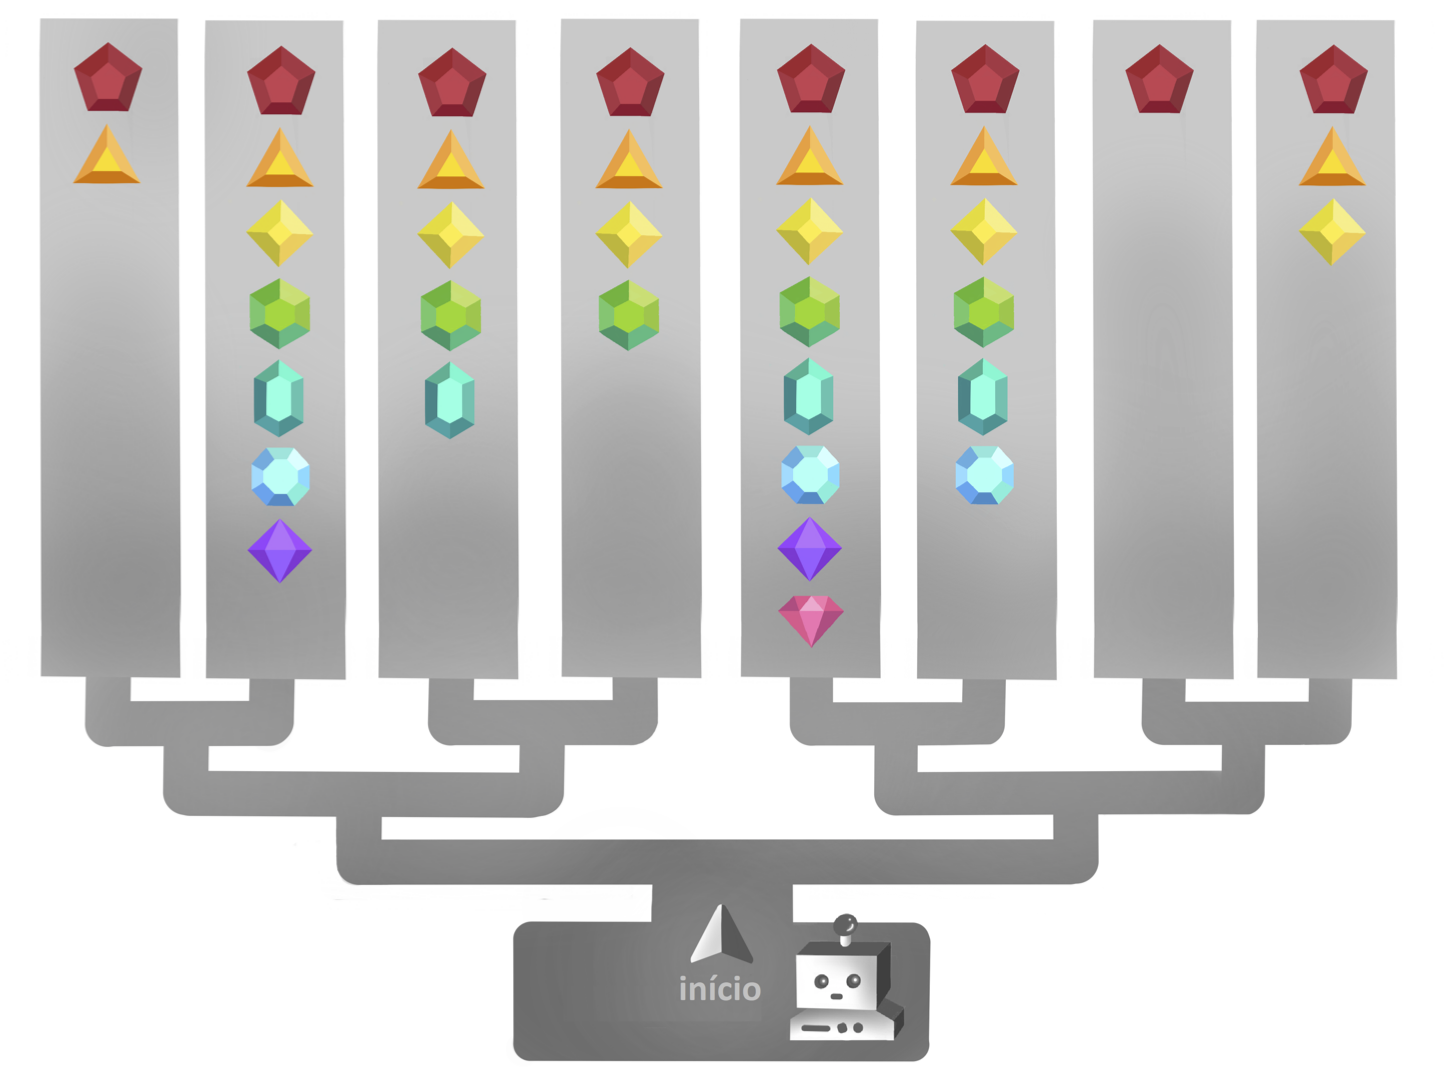
\includegraphics[width=0.6\textwidth]{cp2122t_media/castor11.png}
\caption{
   Labirinto de ``Robôs e Pedras Preciosas".
   \label{fig:labirinto}
}
\end{figure}

\Problema

O \sierp{triângulo de Sierpinski} (Fig.~\ref{fig:sierp1}) é uma figura geométrica
\fractal\ em que um triângulo se subdivide recursivamente em sub-triângulos,
da seguinte forma: considere-se um triângulo rectângulo e
isósceles \ensuremath{\Conid{A}} cujos catetos têm comprimento \ensuremath{\Varid{s}}. A estrutura \fractal\ é
criada desenhando-se três triângulos no interior de \ensuremath{\Conid{A}}, todos eles
rectângulos e isósceles e com catetos de comprimento \ensuremath{\Varid{s}\div \mathrm{2}}. Este passo
é depois repetido para cada um dos triângulos desenhados e assim
sucessivamente (Fig.~\ref{fig:sierp2}).

\begin{figure}[htb]
\begin{center}
	
\includegraphics[width=0.4\textwidth]{cp2122t_media/sierpinski1.png}
\end{center}
  \caption{Um triângulo de Sierpinski com profundidade \ensuremath{\mathrm{4}}.}
  \label{fig:sierp1}
\end{figure}

\begin{figure}[htb]
\begin{center}
	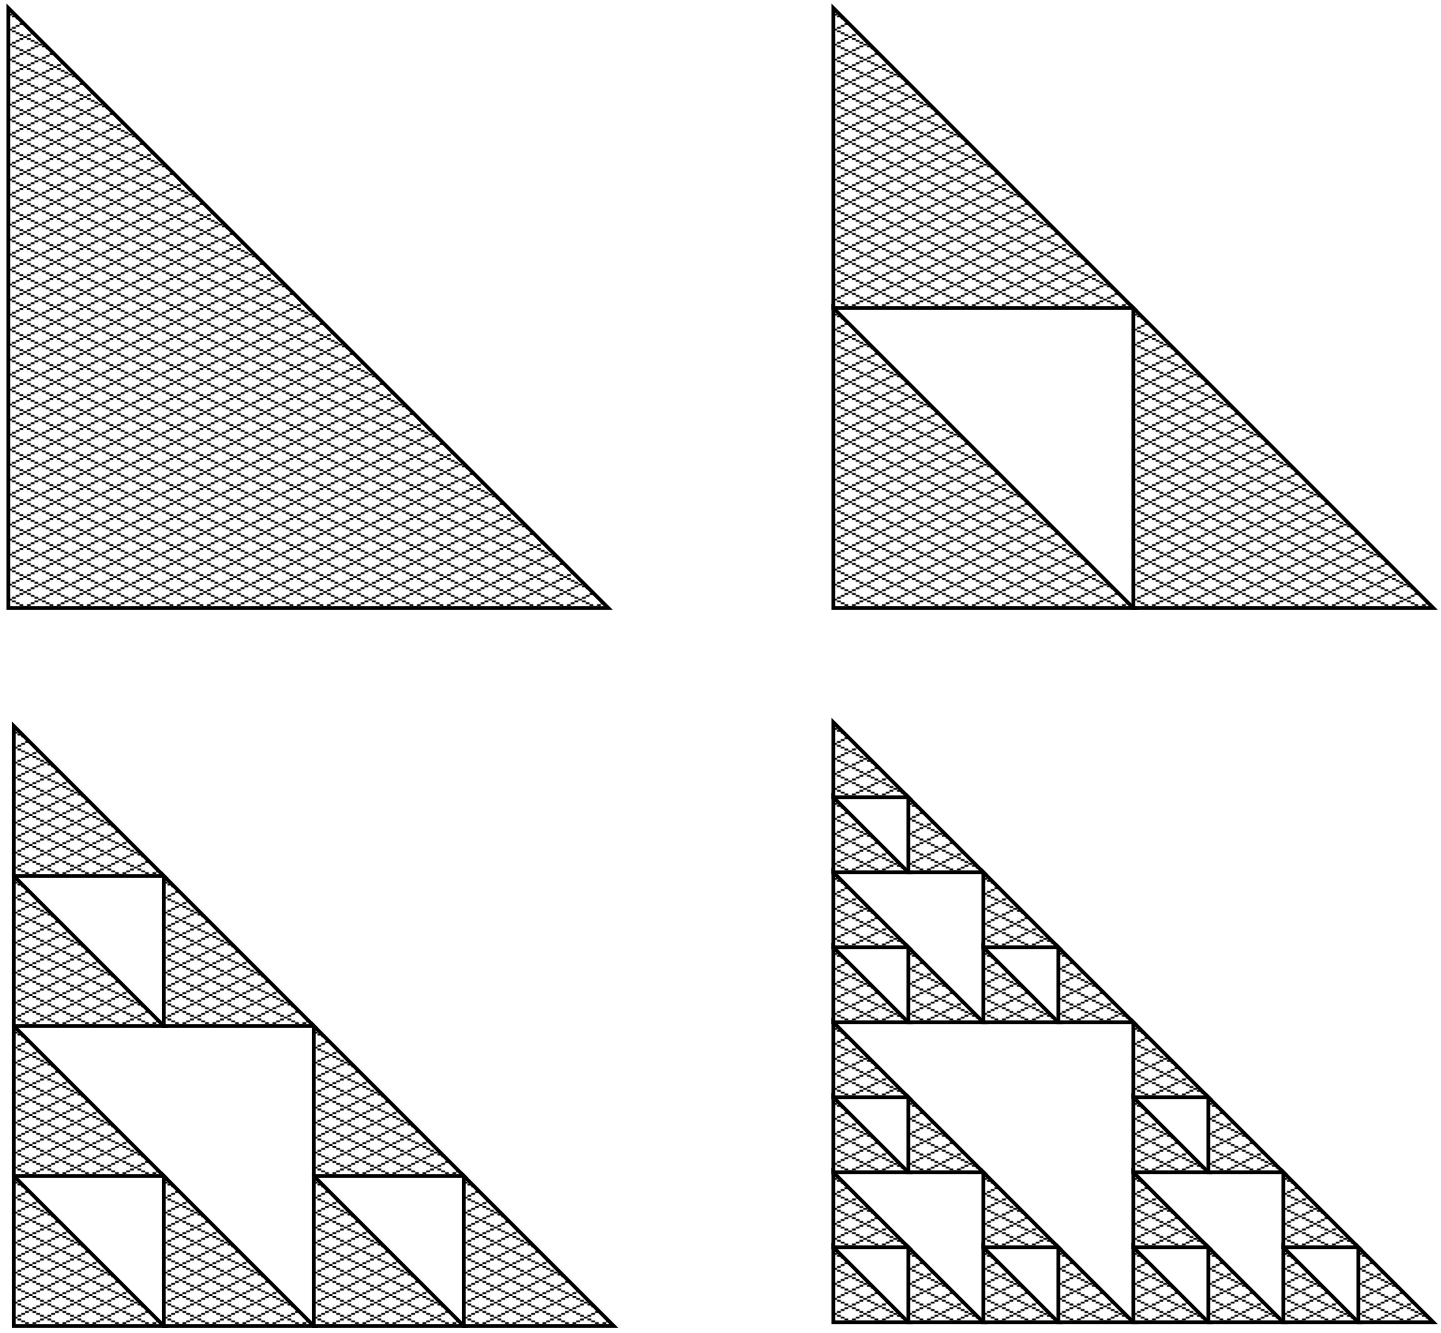
\includegraphics[width=0.6\textwidth]{cp2122t_media/sierpinski2.png}
\end{center}
  \caption{Construção de um triângulo de Sierpinski}
  \label{fig:sierp2}
\end{figure}

Um triângulo de Sierpinski é gerado repetindo-se infinitamente o processo
acima descrito; no entanto para efeitos de visualização é conveniente 
parar o processo recursivo a um determinado nível.

A figura a desenhar é constituída por triângulos todos da mesma dimensão
(por exemplo, no quarto triângulo da Fig.~\ref{fig:sierp2} desenharam-se
27 triângulos). Seja cada triângulo geometricamente descrito pelas coordenadas
do seu vértice inferior esquerdo e o comprimento dos seus catetos:
\begin{hscode}\SaveRestoreHook
\column{B}{@{}>{\hspre}l<{\hspost}@{}}%
\column{E}{@{}>{\hspre}l<{\hspost}@{}}%
\>[B]{}\mathbf{type}\;\Conid{Tri}\mathrel{=}(\Conid{Point},\Conid{Side}){}\<[E]%
\ColumnHook
\end{hscode}\resethooks
onde
\begin{hscode}\SaveRestoreHook
\column{B}{@{}>{\hspre}l<{\hspost}@{}}%
\column{E}{@{}>{\hspre}l<{\hspost}@{}}%
\>[B]{}\mathbf{type}\;\Conid{Side}\mathrel{=}\Conid{Int}{}\<[E]%
\\
\>[B]{}\mathbf{type}\;\Conid{Point}\mathrel{=}(\Conid{Int},\Conid{Int}){}\<[E]%
\ColumnHook
\end{hscode}\resethooks

A estrutura recursiva que suporta a criação de \sierp{triângulos de Sierpinski}
é captada por uma árvore ternária,
\begin{hscode}\SaveRestoreHook
\column{B}{@{}>{\hspre}l<{\hspost}@{}}%
\column{E}{@{}>{\hspre}l<{\hspost}@{}}%
\>[B]{}\mathbf{data}\;\mathsf{LTree3}\;\Varid{a}\mathrel{=}\Conid{Tri}\;\Varid{a}\mid \Conid{Nodo}\;(\mathsf{LTree3}\;\Varid{a})\;(\mathsf{LTree3}\;\Varid{a})\;(\mathsf{LTree3}\;\Varid{a})\;\mathbf{deriving}\;(\Conid{Eq},\Conid{Show}){}\<[E]%
\ColumnHook
\end{hscode}\resethooks
em cujas folhas se irão encontrar os triângulos mais pequenos, todos da
mesma dimensão, que deverão ser desenhados. Apenas estes conterão informação
de carácter geométrico, tendo os nós da árvore um papel exclusivamente estrutural.
Portanto, a informação geométrica guardada em cada folha consiste nas coordenadas
do vértice inferior esquerdo e no cateto do respectivo triângulo. A função
\begin{hscode}\SaveRestoreHook
\column{B}{@{}>{\hspre}l<{\hspost}@{}}%
\column{E}{@{}>{\hspre}l<{\hspost}@{}}%
\>[B]{}\Varid{sierpinski}\mathbin{::}(\Conid{Tri},\Conid{Int})\to [\mskip1.5mu \Conid{Tri}\mskip1.5mu]{}\<[E]%
\\
\>[B]{}\Varid{sierpinski}\mathrel{=}\Varid{folhasSierp}\comp \Varid{geraSierp}{}\<[E]%
\ColumnHook
\end{hscode}\resethooks
recebe a informação do triângulo exterior e a profundidade pretendida,
que funciona como critério de paragem do processo de construção do fractal.
O seu resultado é a lista de triângulos a desenhar.

Esta função é um hilomorfismo do tipo \ensuremath{\mathsf{LTree3}}, i.e.\ a composição de
duas funções: uma que gera \ensuremath{\mathsf{LTree3}}s,
\begin{hscode}\SaveRestoreHook
\column{B}{@{}>{\hspre}l<{\hspost}@{}}%
\column{E}{@{}>{\hspre}l<{\hspost}@{}}%
\>[B]{}\Varid{geraSierp}\mathbin{::}(\Conid{Tri},\Conid{Int})\to \mathsf{LTree3}\;\Conid{Tri}{}\<[E]%
\\
\>[B]{}\Varid{geraSierp}\mathrel{=}\Varid{anaLTree3}\;g_2 {}\<[E]%
\ColumnHook
\end{hscode}\resethooks
e outra que as consome:
\begin{hscode}\SaveRestoreHook
\column{B}{@{}>{\hspre}l<{\hspost}@{}}%
\column{E}{@{}>{\hspre}l<{\hspost}@{}}%
\>[B]{}\Varid{folhasSierp}\mathbin{::}\mathsf{LTree3}\;\Conid{Tri}\to [\mskip1.5mu \Conid{Tri}\mskip1.5mu]{}\<[E]%
\\
\>[B]{}\Varid{folhasSierp}\mathrel{=}\Varid{cataLTree3}\;g_1 {}\<[E]%
\ColumnHook
\end{hscode}\resethooks
Trabalho a realizar:
\begin{enumerate}
\item Desenvolver a biblioteca \emph{pointfree} para o tipo \ensuremath{\mathsf{LTree3}} de forma análoga
      a outras bibliotecas que conhece (\eg\ \BTree, \LTree, etc).
\item Definir os genes \ensuremath{g_1 } e \ensuremath{g_2 } do hilomorfismo \ensuremath{\Varid{sierpinski}}.
\item Correr
\begin{hscode}\SaveRestoreHook
\column{B}{@{}>{\hspre}l<{\hspost}@{}}%
\column{E}{@{}>{\hspre}l<{\hspost}@{}}%
\>[B]{}\Varid{teste}\mathrel{=}\Varid{desenha}\;(\Varid{sierpinski}\;(\Varid{base},\mathrm{3})){}\<[E]%
\ColumnHook
\end{hscode}\resethooks
para verificar a correcta geração de triângulos de Sierpinski em \svg\footnote{\svg,
abreviatura de \emph{Scalable Vector Graphics}, é um dialecto de \xml\ para
computação gráfica. A biblioteca Svg.hs (fornecida) faz uma interface rudimentar
entre \Haskell\ e \svg.}, onde \ensuremath{\Varid{desenha}} é uma função dada no anexo \ref{sec:codigo} que,
para o argumento \ensuremath{\Varid{sierpinski}\;(\Varid{base},\mathrm{3})}, deverá produzir o triângulo colorido da 
Fig.~\ref{fig:sierp1}.\footnote{O resultado é gravado no ficheiro \text{\ttfamily \char95{}\char46{}html}, que pode 
ser visualizado num browser. Poderão ser feitos testes com outros níveis de produndidade.}
\end{enumerate}

\Problema

Os computadores digitais baseiam-se na representação Booleana da informação,
isto é, sob a forma de \emph{bits} que podem ter dois valores, vulg.\ \ensuremath{\mathrm{0}} e \ensuremath{\mathrm{1}}.
Um problema muito frequente é o de os bits se alterarem, devido a ruído ao
nível electrónico. Essas alterações espúrias designam-se \emph{bit-flips}
e podem acontecer a qualquer nível: na transmissão de informação, na gravação
em disco, etc, etc.

Em contraste com essas perturbações, o utilizador de serviços informáticos
raramente dá pela sua presença. Porquê? Porque existe muito trabalho teórico
em correcção dos erros gerados por \emph{bit-flips}, que os permite esconder
do utilizador.

O objectivo desta questão é conseguirmos avaliar experimentalmente o funcionamento
de uma dessas técnicas de correcção de erros, a mais elementar de todas,
chamada \emph{código de repetição}, escrevendo tão pouco código (\Haskell)
quanto possível. Para isso vamos recorrer ao mónade das \emph{distribuições
probabilísticas} (detalhes no apêndice \ref{sec:probabilities}).

Vamos supor que queremos medir a eficácia de um tal código na situação seguinte:
queremos transmitir mensagens que constam exclusivamente de letras maiúsculas,
representadas por 5 bits cada uma segundo o esquema seguinte de codificação,
\begin{hscode}\SaveRestoreHook
\column{B}{@{}>{\hspre}l<{\hspost}@{}}%
\column{E}{@{}>{\hspre}l<{\hspost}@{}}%
\>[B]{}\Varid{enc}\mathbin{::}\Conid{Char}\to \Conid{Bin}{}\<[E]%
\\
\>[B]{}\Varid{enc}\;\Varid{c}\mathrel{=}\Varid{tobin}\;(\Varid{ord}\;\Varid{c}\mathbin{-}\Varid{ord}\;\text{\ttfamily 'A'}){}\<[E]%
\ColumnHook
\end{hscode}\resethooks
e descodificação,
\begin{hscode}\SaveRestoreHook
\column{B}{@{}>{\hspre}l<{\hspost}@{}}%
\column{E}{@{}>{\hspre}l<{\hspost}@{}}%
\>[B]{}\Varid{dec}\mathbin{::}\Conid{Bin}\to \Conid{Char}{}\<[E]%
\\
\>[B]{}\Varid{dec}\;\Varid{b}\mathrel{=}\Varid{chr}\;(\Varid{frombin}\;\Varid{b}\mathbin{+}\Varid{ord}\;\text{\ttfamily 'A'}){}\<[E]%
\ColumnHook
\end{hscode}\resethooks
onde \ensuremath{\Varid{tobin}} e \ensuremath{\Varid{frombin}} são funções dadas no anexo \ref{sec:codigo}. Por exemplo,
\begin{quote}
\ensuremath{\Varid{enc}\;\text{\ttfamily 'A'}\mathrel{=}[\mskip1.5mu \mathrm{0},\mathrm{0},\mathrm{0},\mathrm{0},\mathrm{0}\mskip1.5mu]}
\\
\ensuremath{\Varid{enc}\;\text{\ttfamily 'B'}\mathrel{=}[\mskip1.5mu \mathrm{0},\mathrm{0},\mathrm{0},\mathrm{0},\mathrm{1}\mskip1.5mu]}
\\ $\vdots$ \\
\ensuremath{\Varid{enc}\;\text{\ttfamily 'Z'}\mathrel{=}[\mskip1.5mu \mathrm{1},\mathrm{1},\mathrm{0},\mathrm{0},\mathrm{1}\mskip1.5mu]}
\end{quote}
Embora \ensuremath{\Varid{dec}} e \ensuremath{\Varid{enc}} sejam inversas uma da outra, para o intervalo de \ensuremath{\text{\ttfamily 'A'}}
a \ensuremath{\text{\ttfamily 'Z'}}, deixam de o ser quando, a meio da transmissão, acontecem bit-flips: 

\begin{center}
\unitlength=0.08ex
\linethickness{0.1pt}
\begin{picture}(800.00,110.00)(-160,270)
\put(-170.00,310.00){\ensuremath{\Varid{x}}}
\put( 510.00,310.00){\ensuremath{\Varid{y}}$\not=$ \ensuremath{\Varid{x}}}
\put( 110.00,340.00){(bit-flips)}
\put(-100.00,270.00){\framebox(90,90)[cc]{\ensuremath{\Varid{enc}}}}
\put(350.00,270.00){\framebox(90,90)[cc]{\ensuremath{\Varid{dec}}}}
\put(-150.00,315.00){\vector(1,0){50.00}}
\put( -10.00,315.00){\vector(1,0){50.00}}
\multiput(100.00,315.00)(30,0){5}{.}
\put(300.00,315.00){\vector(1,0){50.00}}
\put(440.00,315.00){\vector(1,0){50.00}}
\end{picture}
\end{center}

Vejamos com quantificar "os estragos". Sabendo-se, por exemplo e por
observação estatística, que a probabilidade de um \ensuremath{\mathrm{0}} virar \ensuremath{\mathrm{1}} é de \ensuremath{\mathrm{4}\mathbin{\%}}
e a de \ensuremath{\mathrm{1}} virar \ensuremath{\mathrm{0}} é de \ensuremath{\mathrm{10}\mathbin{\%}}
\footnote{Estas probabilidades, na prática muito mais baixas, estão inflacionadas
para mais fácil observação.}, simula-se essa informação sobre a forma de
uma função probabilística, em Haskell:
\begin{hscode}\SaveRestoreHook
\column{B}{@{}>{\hspre}l<{\hspost}@{}}%
\column{E}{@{}>{\hspre}l<{\hspost}@{}}%
\>[B]{}\Varid{bflip}\mathbin{::}\Conid{Bit}\to \fun{Dist}\;\Conid{Bit}{}\<[E]%
\\
\>[B]{}\Varid{bflip}\;\mathrm{0}\mathrel{=}\Conid{D}\;[\mskip1.5mu (\mathrm{0},\mathrm{0.96}),(\mathrm{1},\mathrm{0.04})\mskip1.5mu]{}\<[E]%
\\
\>[B]{}\Varid{bflip}\;\mathrm{1}\mathrel{=}\Conid{D}\;[\mskip1.5mu (\mathrm{1},\mathrm{0.90}),(\mathrm{0},\mathrm{0.10})\mskip1.5mu]{}\<[E]%
\ColumnHook
\end{hscode}\resethooks
Agora vamos simular o envio de caracteres. O que devia ser \ensuremath{\Varid{transmit}\mathrel{=}\Varid{dec}\comp \Varid{enc}}
vai ter agora que prever a existência de possíveis bit-flips no meio
da transmissão:
\begin{hscode}\SaveRestoreHook
\column{B}{@{}>{\hspre}l<{\hspost}@{}}%
\column{E}{@{}>{\hspre}l<{\hspost}@{}}%
\>[B]{}\Varid{transmit}\mathrel{=}\Varid{dec'}\comp \Varid{propagate}\;\Varid{bflip}\comp \Varid{enc}{}\<[E]%
\ColumnHook
\end{hscode}\resethooks
Por exemplo, \ensuremath{\Varid{transmit}\;\text{\ttfamily 'H'}} irá dar a seguinte distribuição:
\begin{quote}\small
\begin{tabbing}\ttfamily
~~\char39{}H\char39{}~~67\char46{}2\char37{}\\
\ttfamily ~~\char39{}D\char39{}~~~7\char46{}5\char37{}\\
\ttfamily ~~\char39{}F\char39{}~~~7\char46{}5\char37{}\\
\ttfamily ~~\char39{}G\char39{}~~~7\char46{}5\char37{}\\
\ttfamily ~~\char39{}P\char39{}~~~2\char46{}8\char37{}\\
\ttfamily ~~\char39{}X\char39{}~~~2\char46{}8\char37{}\\
\ttfamily ~~\char39{}E\char39{}~~~0\char46{}8\char37{}\\
\ttfamily ~~\char39{}B\char39{}~~~0\char46{}8\char37{}\\
\ttfamily ~~\char39{}C\char39{}~~~0\char46{}8\char37{}\\
\ttfamily ~~\char39{}L\char39{}~~~0\char46{}3\char37{}\\
\ttfamily ~~\char39{}N\char39{}~~~0\char46{}3\char37{}\\
\ttfamily ~~\char39{}O\char39{}~~~0\char46{}3\char37{}\\
\ttfamily ~~\char39{}T\char39{}~~~0\char46{}3\char37{}\\
\ttfamily ~~\char39{}V\char39{}~~~0\char46{}3\char37{}\\
\ttfamily ~~\char39{}W\char39{}~~~0\char46{}3\char37{}\\
\ttfamily ~~\char39{}\char96{}\char39{}~~~0\char46{}1\char37{}\\
\ttfamily ~~\char39{}A\char39{}~~~0\char46{}1\char37{}
\end{tabbing}
\end{quote}
A saída 'H', que se esperava com \ensuremath{\mathrm{100}\mathbin{\%}} de certeza,
agora só ocorrerá, estatísticamente, com a probabilidade de \ensuremath{\mathrm{67.2}\mathbin{\%}},
consequência dos bit-flips, havendo um âmbito bastante
grande de respostas erradas, mas com probabilidades mais baixas.

\begin{enumerate}
\item \textbf{Trabalho a fazer:} completar a definição do catamorfismo de listas \ensuremath{\Varid{propagate}}.
\end{enumerate}

O que se pode fazer quanto a estes erros de transmissão? Os chamados códigos
de repetição enviam cada bit um número impar de vezes, tipicamente \ensuremath{\mathrm{3}} vezes.
Cada um desses três bits (que na origem são todos iguais) está sujeito
a bit-flips. O que se faz é \emph{votar} no mais frequente --- ver função \ensuremath{v_3 } no anexo.
Se agora a transmissão do \ensuremath{\text{\ttfamily 'H'}} for feita em triplicado,
usando
\begin{hscode}\SaveRestoreHook
\column{B}{@{}>{\hspre}l<{\hspost}@{}}%
\column{E}{@{}>{\hspre}l<{\hspost}@{}}%
\>[B]{}\Varid{transmit3}\mathrel{=}\Varid{dec'}\comp \Varid{propagate3}\;\Varid{bflip3}\comp \Varid{enc}{}\<[E]%
\ColumnHook
\end{hscode}\resethooks
ter-se-á:
\begin{quote}\small
\begin{tabbing}\ttfamily
~Main\char62{}~transmit3~\char39{}H\char39{}\\
\ttfamily ~~\char39{}H\char39{}~~91\char46{}0\char37{}\\
\ttfamily ~~\char39{}F\char39{}~~~2\char46{}6\char37{}\\
\ttfamily ~~\char39{}G\char39{}~~~2\char46{}6\char37{}\\
\ttfamily ~~\char39{}D\char39{}~~~2\char46{}6\char37{}\\
\ttfamily ~~\char39{}P\char39{}~~~0\char46{}4\char37{}\\
\ttfamily ~~\char39{}X\char39{}~~~0\char46{}4\char37{}\\
\ttfamily ~~\char39{}B\char39{}~~~0\char46{}1\char37{}\\
\ttfamily ~~\char39{}C\char39{}~~~0\char46{}1\char37{}\\
\ttfamily ~~\char39{}E\char39{}~~~0\char46{}1\char37{}
\end{tabbing}
\end{quote}
Vê-se que a probabilidade da resposta certa aumentou muito, para \ensuremath{\mathrm{91}\mathbin{\%}},
com redução também do espectro de respostas erradas.

\begin{enumerate}
\setcounter{enumi}{1}
\item \textbf{Trabalho a fazer:} completar a definição do catamorfismo de
listas \ensuremath{\Varid{propagate3}} e da função \ensuremath{\Varid{bflip3}}.
\end{enumerate}

Apesar da sua eficácia, esta técnica de correcção de erros é dispendiosa,
obrigando o envio do triplo dos bits. Isso levou a
comunidade científica a encontrar formas mais sofisticadas para resolver
o mesmo problema sem tal ``overhead". Quem estiver interessado em saber mais
sobre este fascinante tópico poderá começar por visualizar este
\href{https://youtu.be/X8jsijhllIA?t=4}{vídeo} no YouTube.

\part*{Anexos}

\appendix

\section{Documentação para realizar o trabalho}
\label{sec:documentacao}
Para cumprir de forma integrada os objectivos do trabalho vamos recorrer
a uma técnica de programa\-ção dita ``\litp{literária}'' \cite{Kn92},
cujo princípio base é o seguinte:
%
\begin{quote}\em Um programa e a sua documentação devem coincidir.
\end{quote}
%
Por outras palavras, o código fonte e a documentação de um
programa deverão estar no mesmo ficheiro.

O ficheiro \texttt{cp2122t.pdf} que está a ler é já um exemplo de
\litp{programação literária}: foi gerado a partir do texto fonte
\texttt{cp2122t.lhs}\footnote{O sufixo `lhs' quer dizer
\emph{\lhaskell{literate Haskell}}.} que encontrará no
\MaterialPedagogico\ desta disciplina descompactando o ficheiro
\texttt{cp2122t.zip} e executando:
\begin{Verbatim}[fontsize=\small]
    $ lhs2TeX cp2122t.lhs > cp2122t.tex
    $ pdflatex cp2122t
\end{Verbatim}
em que \href{https://hackage.haskell.org/package/lhs2tex}{\texttt\LhsToTeX} é
um pre-processador que faz ``pretty printing''
de código Haskell em \Latex\ e que deve desde já instalar utilizando o
utiliário \href{https://www.haskell.org/cabal/}{cabal} disponível em \href{https://www.haskell.org}{haskell.org}.

Por outro lado, o mesmo ficheiro \texttt{cp2122t.lhs} é executável e contém
o ``kit'' básico, escrito em \Haskell, para realizar o trabalho. Basta executar
\begin{Verbatim}[fontsize=\small]
    $ ghci cp2122t.lhs
\end{Verbatim}

\noindent Abra o ficheiro \texttt{cp2122t.lhs} no seu editor de texto preferido
e verifique que assim é: todo o texto que se encontra dentro do ambiente
\begin{quote}\small\tt
\text{\ttfamily \char92{}begin\char123{}code\char125{}}
\\ ... \\
\text{\ttfamily \char92{}end\char123{}code\char125{}}
\end{quote}
é seleccionado pelo \GHCi\ para ser executado.

\subsection{Como realizar o trabalho}
Este trabalho teórico-prático deve ser realizado por grupos de 3 (ou 4) alunos.
Os detalhes da avaliação (datas para submissão do relatório e sua defesa
oral) são os que forem publicados na \cp{página da disciplina} na \emph{internet}.

Recomenda-se uma abordagem participativa dos membros do grupo em todos os
exercícios do trabalho, para assim poderem responder a qualquer questão colocada
na \emph{defesa oral} do relatório.

Em que consiste, então, o \emph{relatório} a que se refere o parágrafo anterior?
É a edição do texto que está a ser lido, preenchendo o anexo \ref{sec:resolucao}
com as respostas. O relatório deverá conter ainda a identificação dos membros
do grupo de trabalho, no local respectivo da folha de rosto.

Para gerar o PDF integral do relatório deve-se ainda correr os comando seguintes,
que actualizam a bibliografia (com \Bibtex) e o índice remissivo (com \Makeindex),
\begin{Verbatim}[fontsize=\small]
    $ bibtex cp2122t.aux
    $ makeindex cp2122t.idx
\end{Verbatim}
e recompilar o texto como acima se indicou.

No anexo \ref{sec:codigo} disponibiliza-se algum código \Haskell\ relativo
aos problemas que se seguem. Esse anexo deverá ser consultado e analisado
à medida que isso for necessário.

\subsection{Como exprimir cálculos e diagramas em LaTeX/lhs2tex}
Como primeiro exemplo, estudar o texto fonte deste trabalho para obter o
efeito:\footnote{Exemplos tirados de \cite{Ol18}.}
\begin{eqnarray*}
\start
     \ensuremath{\Varid{id}\mathrel{=}\conj{\Varid{f}}{\Varid{g}}}
%
\just\equiv{ universal property }
%
        \ensuremath{\begin{lcbr}\p1\comp \Varid{id}\mathrel{=}\Varid{f}\\\p2\comp \Varid{id}\mathrel{=}\Varid{g}\end{lcbr}}
%
\just\equiv{ identity }
%
        \ensuremath{\begin{lcbr}\p1\mathrel{=}\Varid{f}\\\p2\mathrel{=}\Varid{g}\end{lcbr}}
%
\qed
\end{eqnarray*}

Os diagramas podem ser produzidos recorrendo à \emph{package} \LaTeX\
\href{https://ctan.org/pkg/xymatrix}{xymatrix}, por exemplo:
\begin{eqnarray*}
\xymatrix@C=2cm{
    \ensuremath{\N_0}
           \ar[d]_-{\ensuremath{\cataNat{\Varid{g}}}}
&
    \ensuremath{\mathrm{1}\mathbin{+}\N_0}
           \ar[d]^{\ensuremath{\Varid{id}\mathbin{+}\cataNat{\Varid{g}}}}
           \ar[l]_-{\ensuremath{\mathsf{in}}}
\\
     \ensuremath{\Conid{B}}
&
     \ensuremath{\mathrm{1}\mathbin{+}\Conid{B}}
           \ar[l]^-{\ensuremath{\Varid{g}}}
}
\end{eqnarray*}

\section{Regra prática para a recursividade mútua em \ensuremath{\N_0}}\label{sec:mr}

Nesta disciplina estudou-se como fazer \pd{programação dinâmica} por cálculo,
recorrendo à lei de recursividade mútua.\footnote{Lei (\ref{eq:fokkinga})
em \cite{Ol18}, página \pageref{eq:fokkinga}.}

Para o caso de funções sobre os números naturais (\ensuremath{\N_0}, com functor
\ensuremath{\fun F \;\Conid{X}\mathrel{=}\mathrm{1}\mathbin{+}\Conid{X}}) é fácil derivar-se da lei que foi estudada uma
	\emph{regra de algibeira}
	\label{pg:regra}
que se pode ensinar a programadores que não tenham estudado
\cp{Cálculo de Programas}. Apresenta-se de seguida essa regra, tomando como
exemplo o cálculo do ciclo-\textsf{for} que implementa a função de Fibonacci,
recordar o sistema:
\begin{hscode}\SaveRestoreHook
\column{B}{@{}>{\hspre}l<{\hspost}@{}}%
\column{E}{@{}>{\hspre}l<{\hspost}@{}}%
\>[B]{}\Varid{fib}\;\mathrm{0}\mathrel{=}\mathrm{1}{}\<[E]%
\\
\>[B]{}\Varid{fib}\;(\Varid{n}\mathbin{+}\mathrm{1})\mathrel{=}\Varid{f}\;\Varid{n}{}\<[E]%
\\[\blanklineskip]%
\>[B]{}\Varid{f}\;\mathrm{0}\mathrel{=}\mathrm{1}{}\<[E]%
\\
\>[B]{}\Varid{f}\;(\Varid{n}\mathbin{+}\mathrm{1})\mathrel{=}\Varid{fib}\;\Varid{n}\mathbin{+}\Varid{f}\;\Varid{n}{}\<[E]%
\ColumnHook
\end{hscode}\resethooks
Obter-se-á de imediato
\begin{hscode}\SaveRestoreHook
\column{B}{@{}>{\hspre}l<{\hspost}@{}}%
\column{4}{@{}>{\hspre}l<{\hspost}@{}}%
\column{E}{@{}>{\hspre}l<{\hspost}@{}}%
\>[B]{}\Varid{fib'}\mathrel{=}\p1\comp \for{\Varid{loop}}\ {\Varid{init}}\;\mathbf{where}{}\<[E]%
\\
\>[B]{}\hsindent{4}{}\<[4]%
\>[4]{}\Varid{loop}\;(\Varid{fib},\Varid{f})\mathrel{=}(\Varid{f},\Varid{fib}\mathbin{+}\Varid{f}){}\<[E]%
\\
\>[B]{}\hsindent{4}{}\<[4]%
\>[4]{}\Varid{init}\mathrel{=}(\mathrm{1},\mathrm{1}){}\<[E]%
\ColumnHook
\end{hscode}\resethooks
usando as regras seguintes:
\begin{itemize}
\item	O corpo do ciclo \ensuremath{\Varid{loop}} terá tantos argumentos quanto o número de funções
mutuamente recursivas.
\item	Para as variáveis escolhem-se os próprios nomes das funções, pela ordem
que se achar conveniente.\footnote{Podem obviamente usar-se outros símbolos,
mas numa primeira leitura dá jeito usarem-se tais nomes.}
\item	Para os resultados vão-se buscar as expressões respectivas, retirando
a variável \ensuremath{\Varid{n}}.
\item	Em \ensuremath{\Varid{init}} coleccionam-se os resultados dos casos de base das funções,
pela mesma ordem.
\end{itemize}
Mais um exemplo, envolvendo polinómios do segundo grau $ax^2 + b x + c$ em \ensuremath{\N_0}.
Seguindo o método estudado nas aulas\footnote{Secção 3.17 de \cite{Ol18} e tópico
\href{https://www4.di.uminho.pt/~jno/media/cp/}{Recursividade mútua}
nos vídeos de apoio às aulas teóricas.},
de $f\ x = a x^2 + b x + c$ derivam-se duas funções mutuamente recursivas:
\begin{hscode}\SaveRestoreHook
\column{B}{@{}>{\hspre}l<{\hspost}@{}}%
\column{E}{@{}>{\hspre}l<{\hspost}@{}}%
\>[B]{}\Varid{f}\;\mathrm{0}\mathrel{=}\Varid{c}{}\<[E]%
\\
\>[B]{}\Varid{f}\;(\Varid{n}\mathbin{+}\mathrm{1})\mathrel{=}\Varid{f}\;\Varid{n}\mathbin{+}\Varid{k}\;\Varid{n}{}\<[E]%
\\[\blanklineskip]%
\>[B]{}\Varid{k}\;\mathrm{0}\mathrel{=}\Varid{a}\mathbin{+}\Varid{b}{}\<[E]%
\\
\>[B]{}\Varid{k}\;(\Varid{n}\mathbin{+}\mathrm{1})\mathrel{=}\Varid{k}\;\Varid{n}\mathbin{+}\mathrm{2}\;\Varid{a}{}\<[E]%
\ColumnHook
\end{hscode}\resethooks
Seguindo a regra acima, calcula-se de imediato a seguinte implementação, em Haskell:
\begin{hscode}\SaveRestoreHook
\column{B}{@{}>{\hspre}l<{\hspost}@{}}%
\column{3}{@{}>{\hspre}l<{\hspost}@{}}%
\column{E}{@{}>{\hspre}l<{\hspost}@{}}%
\>[B]{}\Varid{f'}\;\Varid{a}\;\Varid{b}\;\Varid{c}\mathrel{=}\p1\comp \for{\Varid{loop}}\ {\Varid{init}}\;\mathbf{where}{}\<[E]%
\\
\>[B]{}\hsindent{3}{}\<[3]%
\>[3]{}\Varid{loop}\;(\Varid{f},\Varid{k})\mathrel{=}(\Varid{f}\mathbin{+}\Varid{k},\Varid{k}\mathbin{+}\mathrm{2}\mathbin{*}\Varid{a}){}\<[E]%
\\
\>[B]{}\hsindent{3}{}\<[3]%
\>[3]{}\Varid{init}\mathrel{=}(\Varid{c},\Varid{a}\mathbin{+}\Varid{b}){}\<[E]%
\ColumnHook
\end{hscode}\resethooks

\section{O mónade das distribuições probabilísticas} \label{sec:probabilities}
Mónades são functores com propriedades adicionais que nos permitem obter
efeitos especiais em progra\-mação. Por exemplo, a biblioteca \Probability\
oferece um mónade para abordar problemas de probabilidades. Nesta biblioteca,
o conceito de distribuição estatística é captado pelo tipo
\begin{eqnarray}
	\ensuremath{\mathbf{newtype}\;\fun{Dist}\;\Varid{a}\mathrel{=}\Conid{D}\;\{\mskip1.5mu \Varid{unD}\mathbin{::}[\mskip1.5mu (\Varid{a},\Conid{ProbRep})\mskip1.5mu]\mskip1.5mu\}}
	\label{eq:Dist}
\end{eqnarray}
em que \ensuremath{\Conid{ProbRep}} é um real de \ensuremath{\mathrm{0}} a \ensuremath{\mathrm{1}}, equivalente a uma escala de $0$ a
$100 \%$.

Cada par \ensuremath{(\Varid{a},\Varid{p})} numa distribuição \ensuremath{\Varid{d}\mathbin{::}\fun{Dist}\;\Varid{a}} indica que a probabilidade
de \ensuremath{\Varid{a}} é \ensuremath{\Varid{p}}, devendo ser garantida a propriedade de  que todas as probabilidades
de \ensuremath{\Varid{d}} somam $100\%$.
Por exemplo, a seguinte distribuição de classificações por escalões de $A$ a $E$,
\[
\begin{array}{ll}
A & \rule{2mm}{3pt}\ 2\%\\
B & \rule{12mm}{3pt}\ 12\%\\
C & \rule{29mm}{3pt}\ 29\%\\
D & \rule{35mm}{3pt}\ 35\%\\
E & \rule{22mm}{3pt}\ 22\%\\
\end{array}
\]
será representada pela distribuição
\begin{hscode}\SaveRestoreHook
\column{B}{@{}>{\hspre}l<{\hspost}@{}}%
\column{E}{@{}>{\hspre}l<{\hspost}@{}}%
\>[B]{}d_1 \mathbin{::}\fun{Dist}\;\Conid{Char}{}\<[E]%
\\
\>[B]{}d_1 \mathrel{=}\Conid{D}\;[\mskip1.5mu (\text{\ttfamily 'A'},\mathrm{0.02}),(\text{\ttfamily 'B'},\mathrm{0.12}),(\text{\ttfamily 'C'},\mathrm{0.29}),(\text{\ttfamily 'D'},\mathrm{0.35}),(\text{\ttfamily 'E'},\mathrm{0.22})\mskip1.5mu]{}\<[E]%
\ColumnHook
\end{hscode}\resethooks
que o \GHCi\ mostrará assim:
\begin{Verbatim}[fontsize=\small]
'D'  35.0%
'C'  29.0%
'E'  22.0%
'B'  12.0%
'A'   2.0%
\end{Verbatim}
É possível definir geradores de distribuições, por exemplo distribuições \emph{uniformes},
\begin{hscode}\SaveRestoreHook
\column{B}{@{}>{\hspre}l<{\hspost}@{}}%
\column{E}{@{}>{\hspre}l<{\hspost}@{}}%
\>[B]{}d_2 \mathrel{=}\Varid{uniform}\;(\Varid{words}\;\text{\ttfamily \char34 Uma~frase~de~cinco~palavras\char34}){}\<[E]%
\ColumnHook
\end{hscode}\resethooks
isto é
\begin{Verbatim}[fontsize=\small]
     "Uma"  20.0%
   "cinco"  20.0%
      "de"  20.0%
   "frase"  20.0%
"palavras"  20.0%
\end{Verbatim}
distribuição \emph{normais}, eg.\
\begin{hscode}\SaveRestoreHook
\column{B}{@{}>{\hspre}l<{\hspost}@{}}%
\column{E}{@{}>{\hspre}l<{\hspost}@{}}%
\>[B]{}d_3 \mathrel{=}\Varid{normal}\;[\mskip1.5mu \mathrm{10}\mathinner{\ldotp\ldotp}\mathrm{20}\mskip1.5mu]{}\<[E]%
\ColumnHook
\end{hscode}\resethooks
etc.\footnote{Para mais detalhes ver o código fonte de \Probability, que é uma adaptação da
biblioteca \PFP\ (``Probabilistic Functional Programming''). Para quem quiser saber mais
recomenda-se a leitura do artigo \cite{EK06}.} \ensuremath{\fun{Dist}} forma um \textbf{mónade}
cuja unidade é \ensuremath{\Varid{return}\;\Varid{a}\mathrel{=}\Conid{D}\;[\mskip1.5mu (\Varid{a},\mathrm{1})\mskip1.5mu]} e cuja composição de Kleisli é (simplificando a notação)
\begin{hscode}\SaveRestoreHook
\column{B}{@{}>{\hspre}l<{\hspost}@{}}%
\column{3}{@{}>{\hspre}l<{\hspost}@{}}%
\column{E}{@{}>{\hspre}l<{\hspost}@{}}%
\>[3]{}(\Varid{f}\kcomp \Varid{g})\;\Varid{a}\mathrel{=}[\mskip1.5mu (\Varid{y},\Varid{q}\mathbin{*}\Varid{p})\mid (\Varid{x},\Varid{p})\leftarrow \Varid{g}\;\Varid{a},(\Varid{y},\Varid{q})\leftarrow \Varid{f}\;\Varid{x}\mskip1.5mu]{}\<[E]%
\ColumnHook
\end{hscode}\resethooks
em que \ensuremath{\Varid{g}\mathbin{:}\Conid{A}\to \fun{Dist}\;\mathit B} e \ensuremath{\Varid{f}\mathbin{:}\mathit B\to \fun{Dist}\;\mathit C} são funções \textbf{monádicas} que representam
\emph{computações probabilísticas}.

Este mónade é adequado à resolução de problemas de \emph{probabilidades e
estatística} usando programação funcional, de forma elegante e como caso
particular da programação monádica.

\section{Código fornecido}\label{sec:codigo}

\subsection*{Problema 3}

Triângulo de base:
\begin{hscode}\SaveRestoreHook
\column{B}{@{}>{\hspre}l<{\hspost}@{}}%
\column{E}{@{}>{\hspre}l<{\hspost}@{}}%
\>[B]{}\Varid{base}\mathrel{=}((\mathrm{0},\mathrm{0}),\mathrm{32}){}\<[E]%
\ColumnHook
\end{hscode}\resethooks
Desenho de triângulos em \svg:
\begin{hscode}\SaveRestoreHook
\column{B}{@{}>{\hspre}l<{\hspost}@{}}%
\column{E}{@{}>{\hspre}l<{\hspost}@{}}%
\>[B]{}\Varid{desenha}\;\Varid{x}\mathrel{=}\Varid{picd''}\;[\mskip1.5mu \Varid{scale}\;\mathrm{0.44}\;(\mathrm{0},\mathrm{0})\;(\Varid{x}\bind \Varid{tri2svg})\mskip1.5mu]{}\<[E]%
\ColumnHook
\end{hscode}\resethooks
Função que representa cada triângulo em \svg:
\begin{hscode}\SaveRestoreHook
\column{B}{@{}>{\hspre}l<{\hspost}@{}}%
\column{E}{@{}>{\hspre}l<{\hspost}@{}}%
\>[B]{}\Varid{tri2svg}\mathbin{::}\Conid{Tri}\to \Conid{Svg}{}\<[E]%
\\
\>[B]{}\Varid{tri2svg}\;(\Varid{p},\Varid{c})\mathrel{=}(\Varid{red}\comp \Varid{polyg})\;[\mskip1.5mu \Varid{p},\Varid{p}\mathbin{.+}(\mathrm{0},\Varid{c}),\Varid{p}\mathbin{.+}(\Varid{c},\mathrm{0})\mskip1.5mu]{}\<[E]%
\ColumnHook
\end{hscode}\resethooks
\textbf{NB}: o  tipo \ensuremath{\Conid{Svg}} é sinónimo de \ensuremath{\Conid{String}}:
\begin{hscode}\SaveRestoreHook
\column{B}{@{}>{\hspre}l<{\hspost}@{}}%
\column{E}{@{}>{\hspre}l<{\hspost}@{}}%
\>[B]{}\mathbf{type}\;\Conid{Svg}\mathrel{=}\Conid{String}{}\<[E]%
\ColumnHook
\end{hscode}\resethooks

\subsection*{Problema 4}
Funções básicas:
\begin{hscode}\SaveRestoreHook
\column{B}{@{}>{\hspre}l<{\hspost}@{}}%
\column{4}{@{}>{\hspre}l<{\hspost}@{}}%
\column{13}{@{}>{\hspre}l<{\hspost}@{}}%
\column{E}{@{}>{\hspre}l<{\hspost}@{}}%
\>[B]{}\mathbf{type}\;\Conid{Bit}\mathrel{=}\Conid{Int}{}\<[E]%
\\[\blanklineskip]%
\>[B]{}\mathbf{type}\;\Conid{Bin}\mathrel{=}[\mskip1.5mu \Conid{Bit}\mskip1.5mu]{}\<[E]%
\\[\blanklineskip]%
\>[B]{}\mathbf{type}\;\Conid{Bit3}\mathrel{=}(\Conid{Bit},\Conid{Bit},\Conid{Bit}){}\<[E]%
\\[\blanklineskip]%
\>[B]{}\Varid{tobin}\mathrel{=}\Varid{rtrim}\;\mathrm{5}\comp \Varid{pad}\;\mathrm{5}\comp \Varid{dec2bin}{}\<[E]%
\\[\blanklineskip]%
\>[B]{}\Varid{frombin}\mathrel{=}\Varid{bin2dec}\comp \Varid{rtrim}\;\mathrm{5}{}\<[E]%
\\[\blanklineskip]%
\>[B]{}\Varid{bin2dec}\mathbin{::}\Conid{Bin}\to \Conid{Int}{}\<[E]%
\\
\>[B]{}\Varid{bin2dec}\;[\mskip1.5mu \Varid{a}\mskip1.5mu]\mathrel{=}\Varid{a}{}\<[E]%
\\
\>[B]{}\Varid{bin2dec}\;\Varid{b}{}\<[13]%
\>[13]{}\mathrel{=}\Varid{bin2dec}\;(\Varid{init}\;\Varid{b})\mathbin{*}\mathrm{2}\mathbin{+}\Varid{last}\;\Varid{b}{}\<[E]%
\\[\blanklineskip]%
\>[B]{}\Varid{rtrim}\;\Varid{n}\;\Varid{a}\mathrel{=}\Varid{drop}\;(\length \;\Varid{a}\mathbin{-}\Varid{n})\;\Varid{a}{}\<[E]%
\\[\blanklineskip]%
\>[B]{}\Varid{dec2bin}\;\mathrm{0}\mathrel{=}[\mskip1.5mu \mskip1.5mu]{}\<[E]%
\\
\>[B]{}\Varid{dec2bin}\;\Varid{n}\mathrel{=}\Varid{dec2bin}\;\Varid{m}\mathbin{+\!\!\!+}[\mskip1.5mu \Varid{b}\mskip1.5mu]\;\mathbf{where}\;(\Varid{m},\Varid{b})\mathrel{=}(\Varid{n}\div \mathrm{2},\Varid{mod}\;\Varid{n}\;\mathrm{2}){}\<[E]%
\\[\blanklineskip]%
\>[B]{}\Varid{pad}\;\Varid{n}\;\Varid{x}\mathrel{=}\Varid{take}\;\Varid{m}\;\Varid{zeros}\mathbin{+\!\!\!+}\Varid{x}\;\mathbf{where}{}\<[E]%
\\
\>[B]{}\hsindent{4}{}\<[4]%
\>[4]{}\Varid{m}\mathrel{=}\Varid{n}\mathbin{-}\length \;\Varid{x}{}\<[E]%
\\
\>[B]{}\hsindent{4}{}\<[4]%
\>[4]{}\Varid{zeros}\mathrel{=}\mathrm{0}\mathbin{:}\Varid{zeros}{}\<[E]%
\\[\blanklineskip]%
\>[B]{}\Varid{bflips}\mathrel{=}\Varid{propagate}\;\Varid{bflip}{}\<[E]%
\ColumnHook
\end{hscode}\resethooks
Função que vota no bit mais frequente:
\begin{hscode}\SaveRestoreHook
\column{B}{@{}>{\hspre}l<{\hspost}@{}}%
\column{E}{@{}>{\hspre}l<{\hspost}@{}}%
\>[B]{}v_3 \;(\mathrm{0},\mathrm{0},\mathrm{0})\mathrel{=}\mathrm{0}{}\<[E]%
\\
\>[B]{}v_3 \;(\mathrm{0},\mathrm{0},\mathrm{1})\mathrel{=}\mathrm{0}{}\<[E]%
\\
\>[B]{}v_3 \;(\mathrm{0},\mathrm{1},\mathrm{0})\mathrel{=}\mathrm{0}{}\<[E]%
\\
\>[B]{}v_3 \;(\mathrm{0},\mathrm{1},\mathrm{1})\mathrel{=}\mathrm{1}{}\<[E]%
\\
\>[B]{}v_3 \;(\mathrm{1},\mathrm{0},\mathrm{0})\mathrel{=}\mathrm{0}{}\<[E]%
\\
\>[B]{}v_3 \;(\mathrm{1},\mathrm{0},\mathrm{1})\mathrel{=}\mathrm{1}{}\<[E]%
\\
\>[B]{}v_3 \;(\mathrm{1},\mathrm{1},\mathrm{0})\mathrel{=}\mathrm{1}{}\<[E]%
\\
\>[B]{}v_3 \;(\mathrm{1},\mathrm{1},\mathrm{1})\mathrel{=}\mathrm{1}{}\<[E]%
\ColumnHook
\end{hscode}\resethooks
Descodificação monádica:
\begin{hscode}\SaveRestoreHook
\column{B}{@{}>{\hspre}l<{\hspost}@{}}%
\column{E}{@{}>{\hspre}l<{\hspost}@{}}%
\>[B]{}\Varid{dec'}\mathrel{=}\mathsf{fmap}\;\Varid{dec}{}\<[E]%
\ColumnHook
\end{hscode}\resethooks
Para visualização abreviada de distribuições:
\begin{hscode}\SaveRestoreHook
\column{B}{@{}>{\hspre}l<{\hspost}@{}}%
\column{E}{@{}>{\hspre}l<{\hspost}@{}}%
\>[B]{}\Varid{consolidate}\mathbin{::}\Conid{Eq}\;\Varid{a}\Rightarrow \fun{Dist}\;\Varid{a}\to \fun{Dist}\;\Varid{a}{}\<[E]%
\\
\>[B]{}\Varid{consolidate}\mathrel{=}\Conid{D}\comp \Varid{filter}\;\Varid{q}\comp \map \;(\Varid{id}\times\Varid{sum})\comp \Varid{collect}\comp \Varid{unD}\;\mathbf{where}\;\Varid{q}\;(\Varid{a},\Varid{p})\mathrel{=}\Varid{p}\mathbin{>}\mathrm{0.001}{}\<[E]%
\\[\blanklineskip]%
\>[B]{}\Varid{collect}\;\Varid{x}\mathrel{=}\Varid{nub}\;[\mskip1.5mu \Varid{k}\mapsto\Varid{nub}\;[\mskip1.5mu \Varid{d'}\mid (\Varid{k'},\Varid{d'})\leftarrow \Varid{x},\Varid{k'}\equiv \Varid{k}\mskip1.5mu]\mid (\Varid{k},\Varid{d})\leftarrow \Varid{x}\mskip1.5mu]{}\<[E]%
\ColumnHook
\end{hscode}\resethooks

%----------------- Soluções dos alunos -----------------------------------------%

\section{Soluções dos alunos}\label{sec:resolucao}

Os alunos devem colocar neste anexo\footnote{E apenas neste anexo,
i.e, não podem alterar o resto do documento.} as suas soluções para os
exercícios propostos, de acordo com o "layout" que se fornece. Não podem
ser alterados os nomes ou tipos das funções dadas, mas podem ser adicionadas
outras funções auxiliares que sejam necessárias, bem como 
textos, inc.\ diagramas que expliquem como se chegou às soluções encontradas.

Valoriza-se a escrita de \emph{pouco} código que corresponda a soluções
simples e elegantes.

\subsection*{Problema 1} \label{pg:P1}

No problema 1 quer-se mostrar a igualdade entre (aux d) e (loop d). Para o efeito será necessária a lei de recursividade mútua generalizada a 3 funções,
obtida e mostrada no exercício 2 da ficha número 8 desta UC.
\\
\\
A referida lei de recurssividade mútua é a seguinte:

\begin{eqnarray*}
\start%plroblema com os sistemas, uma vez que o lcbr so recebe 2 argumentos e não existe nenhum análogo que receba 3
    \ensuremath{\begin{lcbr}\Varid{f}\comp \mathbf{in}\mathrel{=}\Varid{h}\comp \Conid{F}\;\conj{\Varid{f}}{\conj{\Varid{g}}{\Varid{j}}}\\\Varid{g}\comp \mathbf{in}\mathrel{=}\Varid{k}\comp \Conid{F}\;\conj{\Varid{f}}{\conj{\Varid{g}}{\Varid{j}}}\\\Varid{j}\comp \mathbf{in}\mathrel{=}\Varid{l}\comp \Conid{F}\;\conj{\Varid{f}}{\conj{\Varid{g}}{\Varid{j}}}\end{lcbr}}
%
\equiv
%
    \ensuremath{\Conid{F}\;\conj{\Varid{f}}{\conj{\Varid{g}}{\Varid{j}}}\mathrel{=}\cata{\conj{\Varid{h}}{\conj{\Varid{k}}{\Varid{l}}}}}
\end{eqnarray*}
De forma a mostrar a igualdade pedida, primeiro ter-se-á de definir as funções h, k e l.

Para tal calcula-se o seguinte:
\begin{eqnarray*}
\start
    \ensuremath{\conj{\Varid{q}\;\Varid{d}}{\conj{\Varid{r}\;\Varid{d}}{\Varid{c}\;\Varid{d}}}\mathrel{=}\cata{\conj{\Varid{h}}{\conj{\Varid{k}}{\Varid{l}}}}}
%
\just\equiv{ lei da recursividade mútua (3 funções)}
%
    \ensuremath{\begin{lcbr}(\Varid{q}\;\Varid{d})\comp \mathbf{in}\mathrel{=}\Varid{h}\comp \Conid{F}\;\conj{\Varid{q}\;\Varid{d}}{\conj{\Varid{r}\;\Varid{d}}{\Varid{c}\;\Varid{d}}}\\(\Varid{r}\;\Varid{d})\comp \mathbf{in}\mathrel{=}\Varid{k}\comp \Conid{F}\;\conj{\Varid{q}\;\Varid{d}}{\conj{\Varid{r}\;\Varid{d}}{\Varid{c}\;\Varid{d}}}\\(\Varid{c}\;\Varid{d})\comp \mathbf{in}\mathrel{=}\Varid{l}\comp \Conid{F}\;\conj{\Varid{q}\;\Varid{d}}{\conj{\Varid{r}\;\Varid{d}}{\Varid{c}\;\Varid{d}}}\end{lcbr}}
%
\just\equiv{ def-in , \ensuremath{\Conid{F}\;\Varid{f}\mathrel{=}\Varid{id}\mathbin{+}\Varid{f}} }
%
    \ensuremath{\begin{lcbr}(\Varid{q}\;\Varid{d})\comp \alt{\underline{\mathrm{0}}}{(\succ )}\mathrel{=}\Varid{h}\comp (\Varid{id}\mathbin{+}\conj{\Varid{q}\;\Varid{d}}{\conj{\Varid{r}\;\Varid{d}}{\Varid{c}\;\Varid{d}}})\\(\Varid{r}\;\Varid{d})\comp \alt{\underline{\mathrm{0}}}{(\succ )}\mathrel{=}\Varid{k}\comp (\Varid{id}\mathbin{+}\conj{\Varid{q}\;\Varid{d}}{\conj{\Varid{r}\;\Varid{d}}{\Varid{c}\;\Varid{d}}})\\(\Varid{c}\;\Varid{d})\comp \alt{\underline{\mathrm{0}}}{(\succ )}\mathrel{=}\Varid{l}\comp (\Varid{id}\mathbin{+}\conj{\Varid{q}\;\Varid{d}}{\conj{\Varid{r}\;\Varid{d}}{\Varid{c}\;\Varid{d}}})\end{lcbr}}
%
\just\equiv{ fusão-+ , absorção-+ , \ensuremath{\Varid{h}\mathrel{=}\alt{h_1 }{h_2 },\Varid{k}\mathrel{=}\alt{k_1 }{k_2 },\Varid{l}\mathrel{=}\alt{l_1 }{l_2 }} }
%
    \ensuremath{\begin{lcbr}\alt{(\Varid{q}\;\Varid{d})\comp \underline{\mathrm{0}}}{(\Varid{q}\;\Varid{d})\comp (\succ )}\mathrel{=}\alt{h_1 }{h_2 \comp \conj{\Varid{q}\;\Varid{d}}{\conj{\Varid{r}\;\Varid{d}}{\Varid{c}\;\Varid{d}}}}\\\alt{(\Varid{r}\;\Varid{d})\comp \underline{\mathrm{0}}}{(\Varid{r}\;\Varid{d})\comp (\succ )}\mathrel{=}\alt{k_1 }{k_2 \comp \conj{\Varid{q}\;\Varid{d}}{\conj{\Varid{r}\;\Varid{d}}{\Varid{c}\;\Varid{d}}}}\\\alt{(\Varid{c}\;\Varid{d})\comp \underline{\mathrm{0}}}{(\Varid{c}\;\Varid{d})\comp (\succ )}\mathrel{=}\alt{l_1 }{l_2 \comp \conj{\Varid{q}\;\Varid{d}}{\conj{\Varid{r}\;\Varid{d}}{\Varid{c}\;\Varid{d}}}}\end{lcbr}}
\end{eqnarray*}
Com o intuito do sistema não ficar muito extenso e de difícil leitura, 
modifica-se as equações de modo individual.
\begin{itemize}
\item Equação nº1
\begin{eqnarray*}
\start
    \ensuremath{\alt{(\Varid{q}\;\Varid{d})\comp \underline{\mathrm{0}}}{(\Varid{q}\;\Varid{d})\comp (\succ )}\mathrel{=}\alt{h_1 }{h_2 \comp \conj{\Varid{q}\;\Varid{d}}{\conj{\Varid{r}\;\Varid{d}}{\Varid{c}\;\Varid{d}}}}}
%
\just\equiv{ Eq-+ }
%
    \ensuremath{\begin{lcbr}(\Varid{q}\;\Varid{d})\comp \underline{\mathrm{0}}\mathrel{=}h_1 \\(\Varid{q}\;\Varid{d})\comp (\succ )\mathrel{=}h_2 \comp \conj{\Varid{q}\;\Varid{d}}{\conj{\Varid{r}\;\Varid{d}}{\Varid{c}\;\Varid{d}}}\end{lcbr}}
%
\just\equiv{ igualdade extensional , def-comp , def-split , def-succ}
%
    \ensuremath{\begin{lcbr}\Varid{q}\;\Varid{d}\;\mathrm{0}\mathrel{=}h_1 \;\Varid{n}\\\Varid{q}\;\Varid{d}\;(\Varid{n}\mathbin{+}\mathrm{1})\mathrel{=}h_2 \;(\Varid{q}\;\Varid{d}\;\Varid{n},(\Varid{r}\;\Varid{d}\;\Varid{n},\Varid{c}\;\Varid{d}\;\Varid{n}))\end{lcbr}}
%
\just\equiv{ def-(q d) , 1.ª lei de fusão do condicional , igualdade extensional }
%
    \ensuremath{\begin{lcbr}h_1 \mathrel{=}\underline{\Varid{zero}}\\h_2 \;\Varid{d}\;(\Varid{a},(\Varid{b},\Varid{c}))\mathrel{=}\mathbf{if}\;\Varid{c}\equiv \mathrm{0}\;\mathbf{then}\;\Varid{a}\mathbin{+}\mathrm{1}\;\mathbf{else}\;\Varid{a}\end{lcbr}}
%
\just\equiv{ igualdade extensional , def-cond }
%
    \ensuremath{\begin{lcbr}h_1 \mathrel{=}\underline{\Varid{zero}}\\h_2 \mathrel{=}(\equiv \mathrm{0})\comp \p2\comp \p2\comp \overline{\p2}\to (\succ )\comp \p1\comp \overline{\p2},\p1\comp \overline{\p2}\end{lcbr}}
%
\just\equiv{ \ensuremath{\Varid{h}\mathrel{=}\alt{h_1 }{h_2 }} }
%
    \ensuremath{\Varid{h}\mathrel{=}\alt{\underline{\Varid{zero}}}{(\equiv \mathrm{0})\comp \p2\comp \p2\comp \overline{\p2}\to (\succ )\comp \p1\comp \overline{\p2},\p1\comp \overline{\p2}}}
\end{eqnarray*}
\item Equação nº2
\begin{eqnarray*}
\start
    \ensuremath{\alt{(\Varid{r}\;\Varid{d})\comp \underline{\mathrm{0}}}{(\Varid{r}\;\Varid{d})\comp (\succ )}\mathrel{=}\alt{k_1 }{k_2 \comp \conj{\Varid{q}\;\Varid{d}}{\conj{\Varid{r}\;\Varid{d}}{\Varid{c}\;\Varid{d}}}}}
%
\just\equiv{ Eq-+ }
%
    \ensuremath{\begin{lcbr}(\Varid{r}\;\Varid{d})\comp \underline{\mathrm{0}}\mathrel{=}k_1 \\(\Varid{r}\;\Varid{d})\comp (\succ )\mathrel{=}k_2 \comp \conj{\Varid{q}\;\Varid{d}}{\conj{\Varid{r}\;\Varid{d}}{\Varid{c}\;\Varid{d}}}\end{lcbr}}
%
\just\equiv{ igualdade extensional , def-comp , def-split , def-succ}
%
    \ensuremath{\begin{lcbr}\Varid{r}\;\Varid{d}\;\mathrm{0}\mathrel{=}k_1 \;\Varid{n}\\\Varid{r}\;\Varid{d}\;(\Varid{n}\mathbin{+}\mathrm{1})\mathrel{=}k_2 \;(\Varid{q}\;\Varid{d}\;\Varid{n},(\Varid{r}\;\Varid{d}\;\Varid{n},\Varid{c}\;\Varid{d}\;\Varid{n}))\end{lcbr}}
%
\just\equiv{ def-(r d) , igualdade extensional }
%
    \ensuremath{\begin{lcbr}k_1 \mathrel{=}\underline{\Varid{zero}}\\k_2 \;\Varid{d}\;(\Varid{a},(\Varid{b},\Varid{c}))\mathrel{=}\mathbf{if}\;\Varid{c}\equiv \mathrm{0}\;\mathbf{then}\;\mathrm{0}\;\mathbf{else}\;\mathrm{1}\mathbin{+}\Varid{b}\end{lcbr}}
%
\just\equiv{ igualdade extensional , def-cond , def-const }
%
    \ensuremath{\begin{lcbr}k_1 \mathrel{=}\underline{\Varid{zero}}\\k_2 \mathrel{=}(\equiv \mathrm{0})\comp \p2\comp \p2\comp \overline{\p2}\to \underline{\Varid{zero}},(\succ )\comp \p1\comp \p2\comp \overline{\p2}\end{lcbr}}
%
\just\equiv{ \ensuremath{\Varid{k}\mathrel{=}\alt{k_1 }{k_2 }} }
%
    \ensuremath{\Varid{k}\mathrel{=}\alt{\underline{\Varid{zero}}}{(\equiv \mathrm{0})\comp \p2\comp \p2\comp \overline{\p2}\to \underline{\Varid{zero}},(\succ )\comp \p1\comp \p2\comp \overline{\p2}}}
\end{eqnarray*}
\item Equação nº3
\begin{eqnarray*}
\start
    \ensuremath{\alt{(\Varid{c}\;\Varid{d})\comp \underline{\mathrm{0}}}{(\Varid{c}\;\Varid{d})\comp (\succ )}\mathrel{=}\alt{l_1 }{l_2 \comp \conj{\Varid{q}\;\Varid{d}}{\conj{\Varid{r}\;\Varid{d}}{\Varid{c}\;\Varid{d}}}}}
%
\just\equiv{ Eq-+ }
%
    \ensuremath{\begin{lcbr}(\Varid{c}\;\Varid{d})\comp \underline{\mathrm{0}}\mathrel{=}l_1 \\(\Varid{c}\;\Varid{d})\comp (\succ )\mathrel{=}l_2 \comp \conj{\Varid{q}\;\Varid{d}}{\conj{\Varid{r}\;\Varid{d}}{\Varid{c}\;\Varid{d}}}\end{lcbr}}
%
\just\equiv{ igualdade extensional , def-comp , def-split , def-succ}
%
    \ensuremath{\begin{lcbr}\Varid{c}\;\Varid{d}\;\mathrm{0}\mathrel{=}l_1 \;\Varid{n}\\\Varid{c}\;\Varid{d}\;(\Varid{n}\mathbin{+}\mathrm{1})\mathrel{=}l_2 \;(\Varid{q}\;\Varid{d}\;\Varid{n},(\Varid{r}\;\Varid{d}\;\Varid{n},\Varid{c}\;\Varid{d}\;\Varid{n}))\end{lcbr}}
%
\just\equiv{ def-(c d) , igualdade extensional }
%
    \ensuremath{\begin{lcbr}l_1 \mathrel{=}\underline{\underline{\Varid{d}}}\\l_2 \;\Varid{d}\;(\Varid{a},(\Varid{b},\Varid{c}))\mathrel{=}\mathbf{if}\;\Varid{c}\equiv \mathrm{0}\;\mathbf{then}\;\Varid{d}\;\mathbf{else}\;\Varid{c}\mathbin{-}\mathrm{1}\end{lcbr}}
%
\just\equiv{ igualdade extensional , def-cond }
%
    \ensuremath{\begin{lcbr}l_1 \mathrel{=}\underline{\underline{\Varid{d}}}\\l_2 \mathrel{=}(\equiv \mathrm{0})\comp \p2\comp \p2\comp \overline{\p2}\to \underline{\underline{\Varid{d}}},(\mathbin{-}\mathrm{1})\comp \p2\comp \p2\comp \overline{\p2}\end{lcbr}}
%
\just\equiv{ \ensuremath{\Varid{l}\mathrel{=}\alt{l_1 }{l_2 }} }
%
    \ensuremath{\Varid{l}\mathrel{=}\alt{\underline{\underline{\Varid{d}}}}{(\equiv \mathrm{0})\comp \p2\comp \p2\comp \overline{\p2}\to \underline{\underline{\Varid{d}}},(\mathbin{-}\mathrm{1})\comp \p2\comp \p2\comp \overline{\p2}}}
\end{eqnarray*}
\end{itemize}
Como já definimos \ensuremath{\Varid{h}}, \ensuremath{\Varid{k}} e \ensuremath{\Varid{l}} temos o seguinte:
\begin{eqnarray*}
\start
    \ensuremath{\begin{lcbr}(\Varid{q}\;\Varid{d})\comp \mathbf{in}\mathrel{=}\alt{\underline{\Varid{zero}}}{h_1 }\comp \Conid{F}\;\conj{\Varid{q}\;\Varid{d}}{\conj{\Varid{r}\;\Varid{d}}{\Varid{c}\;\Varid{d}}}\\(\Varid{r}\;\Varid{d})\comp \mathbf{in}\mathrel{=}\alt{\underline{\Varid{zero}}}{k_2 }\comp \Conid{F}\;\conj{\Varid{q}\;\Varid{d}}{\conj{\Varid{r}\;\Varid{d}}{\Varid{c}\;\Varid{d}}}\\(\Varid{c}\;\Varid{d})\comp \mathbf{in}\mathrel{=}\alt{\underline{\underline{\Varid{d}}}}{l_2 }\comp \Conid{F}\;\conj{\Varid{q}\;\Varid{d}}{\conj{\Varid{r}\;\Varid{d}}{\Varid{c}\;\Varid{d}}}\end{lcbr}}
%
\just\equiv{ fokkinga }
%
    \ensuremath{\conj{(\Varid{q}\;\Varid{d})}{\conj{(\Varid{r}\;\Varid{d})}{(\Varid{c}\;\Varid{d})}}\mathrel{=}}
    \ensuremath{\cata{\conj{\alt{\underline{\Varid{zero}}}{h_2 }}{\conj{\alt{\underline{\Varid{zero}}}{k_2 }}{\alt{\underline{\underline{\Varid{d}}}}{l_2 }}}}}
%
\just\equiv{ lei da troca }
%
    \ensuremath{\conj{(\Varid{q}\;\Varid{d})}{\conj{(\Varid{r}\;\Varid{d})}{(\Varid{c}\;\Varid{d})}}\mathrel{=}\cata{\conj{\alt{\underline{\Varid{zero}}}{h_2 }}{\alt{\conj{\underline{\Varid{zero}}}{\underline{\underline{\Varid{d}}}}}{\conj{k_2 }{l_2 }}}}}
%
\just\equiv{ lei da troca }
%
    \ensuremath{\conj{(\Varid{q}\;\Varid{d})}{\conj{(\Varid{r}\;\Varid{d})}{(\Varid{c}\;\Varid{d})}}\mathrel{=}\cata{\alt{\conj{\underline{\Varid{zero}}}{\conj{\underline{\Varid{zero}}}{\underline{\underline{\Varid{d}}}}}}{\conj{h_2 }{\conj{k_2 }{l_2 }}}}}
%
\just\equiv{ igualdade extensional, def-split, def-const}
%
    \ensuremath{\conj{(\Varid{q}\;\Varid{d})}{\conj{(\Varid{r}\;\Varid{d})}{(\Varid{c}\;\Varid{d})}}\mathrel{=}\cata{\alt{\underline{(\Varid{zero},(\Varid{zero},\underline{\Varid{d}}))}}{\conj{h_2 }{\conj{k_2 }{l_2 }}}}}
%
\just\equiv{ def for }
%
    \ensuremath{\conj{(\Varid{q}\;\Varid{d})}{\conj{(\Varid{r}\;\Varid{d})}{(\Varid{c}\;\Varid{d})}}\mathrel{=}\for{\conj{h_2 }{\conj{k_2 }{l_2 }}}\ {(\mathrm{0},(\mathrm{0},\Varid{d}))}}
\end{eqnarray*}
Prova-se, agora, a igualdade entre (g d) e o split que se encontra no ciclo for obtido.
\begin{eqnarray*}
\start
    \ensuremath{(\Varid{g}\;\Varid{d})\mathrel{=}\conj{h_2 }{\conj{k_2 }{l_2 }}}
%
\just\equiv{ igualdade extensional, def-split }
%
    \ensuremath{\Varid{g}\;\Varid{d}\;(\Varid{q},(\Varid{r},\Varid{c}))\mathrel{=}(h_2 \;\Varid{d}\;(\Varid{q},(\Varid{r},\Varid{c})),(k_2 \;\Varid{d}\;(\Varid{q},(\Varid{r},\Varid{c})),l_2 \;\Varid{d}\;(\Varid{q},(\Varid{r},\Varid{c}))))}
%
\just\equiv{ def \ensuremath{\Varid{p}\to \Varid{f},\Varid{g}},  def succ, def-const, def-proj, curry }
%
    \ensuremath{\begin{lcbr}\Varid{g}\;\Varid{d}\;(\Varid{q},(\Varid{r},\Varid{c}))\mathrel{=}(\equiv \mathrm{0})\;\Varid{c}\Rightarrow(\Varid{q}\mathbin{+}\mathrm{1},(\mathrm{0},\Varid{d}))\\\Varid{g}\;\Varid{d}\;(\Varid{q},(\Varid{r},\Varid{c}))\mathrel{=}\neg \;(\equiv \mathrm{0})\;\Varid{c}\Rightarrow(\Varid{q},(\Varid{r}\mathbin{+}\mathrm{1},\Varid{c}\mathbin{-}\mathrm{1}))\end{lcbr}}
%
\equiv
%
    \ensuremath{\begin{lcbr}\Varid{g}\;\Varid{d}\;(\Varid{q},(\Varid{r},\mathrm{0}))\mathrel{=}(\Varid{q}\mathbin{+}\mathrm{1},(\mathrm{0},\Varid{d}))\\\Varid{g}\;\Varid{d}\;(\Varid{q},(\Varid{r},\Varid{c}\mathbin{+}\mathrm{1}))\mathrel{=}(\Varid{q},(\Varid{r}\mathbin{+}\mathrm{1},\Varid{c}))\end{lcbr}}
\end{eqnarray*}
Assim, pode-se concluir que (aux d) é igual a (loop d).
\subsection*{Problema 2}

Este desafio foi muito interessante de desenvolver, tanto em código como o próprio processo evolutivo do pensamento envolvido para toda a resolução e estruturação do problema.
\\
\\
Para resolver este desafio a ideia "imediata" que surgiu foi, uma vez que os objetivos de cada um são conhecidos por ambos e além disso existe uma ordem definida para as jogadas, então é possível que cada um consiga prever as jogada do outro. Ou seja, já que a Alice e o Bob jogam à vez, esta visão transmitiu, nesse instante, a ideia de recursividade mútua, onde a Alice prevê as jogadas do Bob e vice-versa. 
\\
\\
Para esse efeito codificou-se primeiro as funções \emph{alice}, \emph{bob} e \emph{both} e só depois (através das leis de recursividade mútua) definiu-se \emph{both} como catamorfismo. A função \emph{alice} foi definida de modo a obter o número máximo de pedras preciosas de entre as possíveis escolhas posteriores de Bob, sendo o seu objetivo oposto ao de Alice, ou seja, o de obter o número mínimo de pedras preciosas. Com o mesmo raciocínio definou-se \emph{bob} que adquire o mínimo de pedras preciosas de entre as diversas escolhas que a Alice poderá vir a tomar. \emph{both} foi definida de modo a ser possível observar os diferentes resultados obtidos por ambas as partes aquando do jogo ser inicializado por Alice ou por Bob.

\begin{hscode}\SaveRestoreHook
\column{B}{@{}>{\hspre}l<{\hspost}@{}}%
\column{E}{@{}>{\hspre}l<{\hspost}@{}}%
\>[B]{}\Varid{alice}\mathbin{::}\Conid{Ord}\;\Varid{c}\Rightarrow {\LTree}\;\Varid{c}\to \Varid{c}{}\<[E]%
\\
\>[B]{}\Varid{alice}\;(\Conid{Leaf}\;\Varid{x})\mathrel{=}\Varid{x}{}\<[E]%
\\
\>[B]{}\Varid{alice}\;(\Conid{Fork}\;(\Varid{e},\Varid{d}))\mathrel{=}\Varid{max}\;(\Varid{bob}\;\Varid{e})\;(\Varid{bob}\;\Varid{d}){}\<[E]%
\\[\blanklineskip]%
\>[B]{}\Varid{bob}\mathbin{::}\Conid{Ord}\;\Varid{c}\Rightarrow {\LTree}\;\Varid{c}\to \Varid{c}{}\<[E]%
\\
\>[B]{}\Varid{bob}\;(\Conid{Leaf}\;\Varid{x})\mathrel{=}\Varid{x}{}\<[E]%
\\
\>[B]{}\Varid{bob}\;(\Conid{Fork}\;(\Varid{e},\Varid{d}))\mathrel{=}\Varid{min}\;(\Varid{alice}\;\Varid{e})\;(\Varid{alice}\;\Varid{d}){}\<[E]%
\\[\blanklineskip]%
\>[B]{}\Varid{both}\mathbin{::}\Conid{Ord}\;\Varid{d}\Rightarrow {\LTree}\;\Varid{d}\to (\Varid{d},\Varid{d}){}\<[E]%
\\
\>[B]{}\Varid{both}\;\Varid{t}\mathrel{=}(\Varid{alice}\;\Varid{t},\Varid{bob}\;\Varid{t}){}\<[E]%
\ColumnHook
\end{hscode}\resethooks
\\
\\
Depois de definidas as três funções e para ser possível a utilização das leis da recursividade mútua, foi necessária a definição de uma função h e k. Por essa razão, calculou-se as mesmas a partir da definição de \emph{alice} e de \emph{bob} acima referidas como se pode ver a seguir.
\\
\\
\begin{eqnarray*}
\start
    \ensuremath{\begin{lcbr}\Varid{alice}\;(\Conid{Leaf}\;\Varid{x})\mathrel{=}\Varid{x}\\\Varid{alice}\;(\Conid{Fork}\;(\Varid{e},\Varid{d}))\mathrel{=}\Varid{max}\;(\Varid{bob}\;\Varid{e})\;(\Varid{bob}\;\Varid{d})\end{lcbr}}
%
\just\equiv{ uncurry }
%
    \ensuremath{\begin{lcbr}\Varid{alice}\;(\Conid{Leaf}\;\Varid{x})\mathrel{=}\Varid{x}\\\Varid{alice}\;(\Conid{Fork}\;(\Varid{e},\Varid{d}))\mathrel{=}\uncurry{\Varid{max}}\;(\Varid{bob}\;\Varid{e},\Varid{bob}\;\Varid{d})\end{lcbr}}
%
\just\equiv{ def-x, def-comp, def-id, igualdade extensional }
%
    \ensuremath{\begin{lcbr}\Varid{alice}\comp \Conid{Leaf}\mathrel{=}\Varid{id}\\\Varid{alice}\comp \Conid{Fork}\mathrel{=}\uncurry{\Varid{max}}\comp (\Varid{bob}\times\Varid{bob})\end{lcbr}}
%
\just\equiv{ eq-+ }
%
    \ensuremath{\alt{\Varid{alice}\comp \Conid{Leaf}}{\Varid{alice}\comp \Conid{Fork}}\mathrel{=}\alt{\Varid{id}}{\uncurry{\Varid{max}}\comp (\Varid{bob}\times\Varid{bob})}}
%
\just\equiv{ fusão-+ , cancelamento-x }
%
    \ensuremath{\Varid{alice}\comp \alt{\Conid{Leaf}}{\Conid{Fork}}\mathrel{=}\alt{\Varid{id}}{\uncurry{\Varid{max}}\comp (\p2\comp \conj{\Varid{alice}}{\Varid{bob}}\times\p2\comp \conj{\Varid{alice}}{\Varid{bob}})}}
%
\just\equiv{ functor-x , def-in }
%
    \ensuremath{\Varid{alice}\comp \mathbf{in}\mathrel{=}\alt{\Varid{id}}{\uncurry{\Varid{max}}\comp (\p2\times\p2)\comp (\conj{\Varid{alice}}{\Varid{bob}}\times\conj{\Varid{alice}}{\Varid{bob}})}}
%
\just\equiv{ absorção-+ , natural-id }
%
    \ensuremath{\Varid{alice}\comp \mathbf{in}\mathrel{=}\alt{\Varid{id}}{\uncurry{\Varid{max}}\comp (\p2\times\p2)}\comp (\Varid{id}\mathbin{+}\conj{\Varid{alice}}{\Varid{bob}}\times\conj{\Varid{alice}}{\Varid{bob}})}
%
\just\equiv{ \ensuremath{\Conid{F}\;\Varid{f}\mathrel{=}\Varid{id}\mathbin{+}\Varid{f}\times\Varid{f}} }
%
    \ensuremath{\Varid{alice}\comp \mathbf{in}\mathrel{=}\alt{\Varid{id}}{\uncurry{\Varid{max}}\comp (\p2\times\p2)}\comp \Conid{F}\;\conj{\Varid{alice}}{\Varid{bob}}}
\end{eqnarray*}
Logo, h= \ensuremath{\alt{\Varid{id}}{\uncurry{\Varid{max}}\comp (\p2\times\p2)}}
\\
\\
De modo análogo, a partir da definição acima indicada de \emph{bob}, e usando as mesmas leis, obtém-se
\\
k = \ensuremath{\alt{\Varid{id}}{\uncurry{\Varid{min}}\comp (\p1\times\p1)}}.
\\
\\
Depois de h e k definidas, tem-se o seguinte.
\begin{eqnarray*}
\start
    \ensuremath{\begin{lcbr}\Varid{alice}\comp \mathbf{in}\mathrel{=}\alt{\Varid{id}}{\uncurry{\Varid{max}}\comp (\p2\times\p2)}\comp \Conid{F}\;\conj{\Varid{alice}}{\Varid{bob}}\\\Varid{bob}\comp \mathbf{in}\mathrel{=}\alt{\Varid{id}}{\uncurry{\Varid{min}}\comp (\p1\times\p1)}\comp \Conid{F}\;\conj{\Varid{alice}}{\Varid{bob}}\end{lcbr}}
    )
%
\just\equiv{ fokkinga }
%
    \ensuremath{\conj{\Varid{alice}}{\Varid{bob}}\mathrel{=}\cata{\conj{\alt{\Varid{id}}{\uncurry{\Varid{max}}\comp (\p2\times\p2)}}{\alt{\Varid{id}}{\uncurry{\Varid{min}}\comp (\p1\times\p1)}}}}
\end{eqnarray*}
Tendo como resultado a função \emph{both} definida como catamorfismo de LTree's.

\subsection*{Problema 3}

O raciocínio seguido nesta primeira parte do problema depende das diferentes funções definidas, pelo que vão ser explicadas separadamente.
\begin{itemize}
\item O \emph{inLTree3} recebe um Either onde a sua segunda componente é um par e o seu primeiro elemento também o é, ou seja, é do tipo ((\ensuremath{\mathsf{LTree3}} a,\ensuremath{\mathsf{LTree3}} a),\ensuremath{\mathsf{LTree3}} a). Foi assim definida uma vez que, em haskell, não é possível a existência de um tuplo com três elementos. Esta função devolve uma LTree3. Para tal ser executado, \emph{inLTree3} é formado pelos construtures do tipo \ensuremath{\mathsf{LTree3}}, sendo que para ser possível a utilização de \ensuremath{\Conid{Nodo}} é necessária a realização do uncurry duas vezes consecutivas.
\item Relativamente à função \emph{outLTree3} o mesmo tipo de pensamento de \emph{inLTree3} foi aqui utilizado. Neste caso, recebe uma \ensuremath{\mathsf{LTree3}} e devolve um Either. O modo de funcionamento é caso seja de tipo \ensuremath{\Conid{Tri}} devolve-o, caso contrário agrupa as três \ensuremath{\mathsf{LTree3}}'s num par de um par de modo a ser compatível com o tipo de saída da segunda componente do Either.
\item A \emph{baseLTree3} é o bifuntor deste tipo (\ensuremath{\mathsf{LTree3}}), havendo dois parâmetros diferentes: o \ensuremath{\Conid{Tri}} e a \ensuremath{\mathsf{LTree3}}.
\item \emph{recLTree3} é o functor de \ensuremath{\mathsf{LTree3}}, ou seja, é o bifuntor de id e de um f que irá receber.
\item O funcionamento das funções \emph{cataLTree3}, \emph{anaLTree3} e \emph{hyloLTree3} é a sua definição recorrendo a funções previamente definidas do mesmo tipo.
\end{itemize}
A biblioteca de \ensuremath{\mathsf{LTree3}} é:
\begin{hscode}\SaveRestoreHook
\column{B}{@{}>{\hspre}l<{\hspost}@{}}%
\column{E}{@{}>{\hspre}l<{\hspost}@{}}%
\>[B]{}\Varid{inLTree3}\mathrel{=}\alt{\Conid{Tri}}{\uncurry{\uncurry{\Conid{Nodo}}}}{}\<[E]%
\\[\blanklineskip]%
\>[B]{}\Varid{outLTree3}\;(\Conid{Tri}\;\Varid{t})\mathrel{=}i_1\;\Varid{t}{}\<[E]%
\\
\>[B]{}\Varid{outLTree3}\;(\Conid{Nodo}\;\Varid{a}\;\Varid{b}\;\Varid{c})\mathrel{=}i_2\;((\Varid{a},\Varid{b}),\Varid{c}){}\<[E]%
\\[\blanklineskip]%
\>[B]{}\Varid{baseLTree3}\;\Varid{f}\;\Varid{g}\mathrel{=}\Varid{f}+(\Varid{g}\times\Varid{g})\times\Varid{g}{}\<[E]%
\\[\blanklineskip]%
\>[B]{}\Varid{recLTree3}\;\Varid{f}\mathrel{=}\Varid{id}+(\Varid{f}\times\Varid{f})\times\Varid{f}{}\<[E]%
\\[\blanklineskip]%
\>[B]{}\Varid{cataLTree3}\;\Varid{f}\mathrel{=}\Varid{f}\comp (\Varid{recLTree3}\;(\Varid{cataLTree3}\;\Varid{f}))\comp \Varid{outLTree3}{}\<[E]%
\\[\blanklineskip]%
\>[B]{}\Varid{anaLTree3}\;\Varid{f}\mathrel{=}\Varid{inLTree3}\comp (\Varid{recLTree3}\;(\Varid{anaLTree3}\;\Varid{f}))\comp \Varid{f}{}\<[E]%
\\[\blanklineskip]%
\>[B]{}\Varid{hyloLTree3}\;\Varid{f}\;\Varid{g}\mathrel{=}\Varid{cataLTree3}\;\Varid{f}\comp \Varid{anaLTree3}\;\Varid{g}{}\<[E]%
\ColumnHook
\end{hscode}\resethooks
\\
\\
Esta segunda parte do problema 3, foi realizada através de gráficos. De modo a
 definir o gene do catamorfismo foi feito o seu diagrama (indicado abaixo).
\\
\begin{eqnarray*}
\xymatrix@C=3cm@R=1.7cm{
    \ensuremath{\mathsf{LTree3}\;\Conid{Tri}}
           \ar[d]_-{\ensuremath{\Varid{folhasSierp}}}
           \ar@/_2pc/[r]_-{\ensuremath{\Varid{out}}}
&
    \ensuremath{\Conid{Tri}\mathbin{+}((\mathsf{LTree3}\;\Conid{Tri}\times\mathsf{LTree3}\;\Conid{Tri})\times\mathsf{LTree3}\;\Conid{Tri})}
           \ar[d]^{\ensuremath{\Varid{id}\mathbin{+}((\Varid{folhasSierp}\times\Varid{folhasSierp})\times\Varid{folhasSierp})}}
           \ar@/_2pc/[l]_-{\ensuremath{\mathbf{in}}}
\\
     \ensuremath{\Conid{Tri}\mathbin{*}}
&
     \ensuremath{\Conid{Tri}\mathbin{+}((\Conid{Tri}\mathbin{*}\times\Conid{Tri}\mathbin{*})\times\Conid{Tri}\mathbin{*})}
           \ar[l]^-{\ensuremath{g_1 }}
}
\end{eqnarray*}
\\
\\
Nesse diagrama pode-se observar os diferentes tipos de entrada e de saída de \emph{folhasSierp}, tal como de \ensuremath{g_1 }. Deste modo, é percetível que este será um 
Either, onde na primeira componente estará uma função que transforma um Tri numa 
lista com esse mesmo Tri. Na segunda componente estará uma função que junta as
 diferentes listas originadas de três \ensuremath{\mathsf{LTree3}}'s numa só. Analisando o tipo que o
 gene do catamorfismo recebe concluiu-se que será a composta entre duas funções,
 uma que junta o primeiro elemento do par de listas numa só lista e outra que 
junta a lista resultante com o segundo elemento do par inicial. Esta análise está representada através do diagrama que se segue.
\\
%diagrama extra dos tipos
\begin{eqnarray*}
\xymatrix@C=2cm{
    \ensuremath{((\Conid{Tri}\mathbin{*}\times\Conid{Tri}\mathbin{*})\times\Conid{Tri}\mathbin{*})}
           \ar[d]^-{\ensuremath{\uncurry{(\mathbin{+\!\!\!+})}\times\Varid{id}}}
\\
    \ensuremath{\Conid{Tri}\mathbin{*}\times\Conid{Tri}\mathbin{*}}
           \ar[d]^{\ensuremath{\uncurry{(\mathbin{+\!\!\!+})}}}
\\
    \ensuremath{\Conid{Tri}\mathbin{*}}
}
\end{eqnarray*}
\\
\\
No sentido de se definir o gene do anamorfismo, foi, também, realizado o seu diagrama, como se pode ver de seguida.

\begin{eqnarray*}
\xymatrix@C=3cm@R=1.7cm{
    \ensuremath{(\Conid{Tri}\times\N_0)}
           \ar[d]_-{\ensuremath{\Varid{geraSierp}}}
           \ar[r]_-{\ensuremath{g_2 }}
&
    \ensuremath{\Conid{Tri}\mathbin{+}(((\Conid{Tri}\times\N_0)\times(\Conid{Tri}\times\N_0))\times(\Conid{Tri}\times\N_0))}
           \ar[d]^{\ensuremath{\Varid{id}\mathbin{+}((\Varid{geraSierp}\times\Varid{geraSierp})\times\Varid{geraSierp})}}
\\
     \ensuremath{\mathsf{LTree3}\;\Conid{Tri}}
            \ar@/_2pc/[r]_-{\ensuremath{\Varid{out}}}
&
     \ensuremath{\Conid{Tri}\mathbin{+}((\mathsf{LTree3}\;\Conid{Tri}\times\mathsf{LTree3}\;\Conid{Tri})\times\mathsf{LTree3}\;\Conid{Tri})}
           \ar@/_2pc/[l]_-{\ensuremath{\mathbf{in}}}
}
\end{eqnarray*}
Neste diagrama pode-se observar os tipos recebidos e devolvidos pelas diferentes
 funções, nomeadamente de \ensuremath{g_2 }, isto é, do gene do anamorfismo. Como o tipo
 recebido é um par e o devolvido é um Either, é imediata a necessidade da 
utilização das funções \ensuremath{i_1} e \ensuremath{i_2}. Caso o número referente à profundidade for 0 o gene vai devolver o triângulo. Caso contrário, este, de modo recursivo, vai criar os três triângulos com os respetivos vértices e tamanho dos catetos, diminuindo um ao nível de profundidade. A seguir explicam-se como se formam os diferentes triângulos (através de \ensuremath{\Varid{t1}}, \ensuremath{\Varid{t2}} e \ensuremath{\Varid{t3}}).
\\
\\
\ensuremath{\Varid{t1}} cria um triângulo somando à coordenada x metade do tamanho do cateto do triângulo da profundidade superior e, por sua vez, dividindo o tamanho do cateto por dois. 
\\
\\
\ensuremath{\Varid{t2}} modifica a coordenada y tal como é feito em \ensuremath{\Varid{t1}} e dividindo, também, o tamanho do cateto por dois, de forma a criar outro triângulo.
\\
\\
Por último, \ensuremath{\Varid{t3}} cria o triângulo cujas coordenadas se mantêm e apenas se reduz o tamanho do cateto. 
\\
\\
Os genes do hilomorfismo \ensuremath{\Varid{sierpinski}} são:
\begin{hscode}\SaveRestoreHook
\column{B}{@{}>{\hspre}l<{\hspost}@{}}%
\column{6}{@{}>{\hspre}l<{\hspost}@{}}%
\column{E}{@{}>{\hspre}l<{\hspost}@{}}%
\>[B]{}g_1 \mathrel{=}\alt{\Varid{singl}}{(\mathsf{conc})\comp ((\mathsf{conc})\times\Varid{id})}{}\<[E]%
\\[\blanklineskip]%
\>[B]{}g_2 \;(\Varid{t},\mathrm{0})\mathrel{=}i_1\;\Varid{t}{}\<[E]%
\\
\>[B]{}g_2 \;(((\Varid{x},\Varid{y}),\Varid{s}),\Varid{n}\mathbin{+}\mathrm{1})\mathrel{=}i_2\;((\Varid{t1},\Varid{t2}),\Varid{t3})\;\mathbf{where}{}\<[E]%
\\
\>[B]{}\hsindent{6}{}\<[6]%
\>[6]{}\Varid{t1}\mathrel{=}(((\Varid{x}\mathbin{+}\Varid{s}\div \mathrm{2},\Varid{y}),\Varid{s}\div \mathrm{2}),\Varid{n}){}\<[E]%
\\
\>[B]{}\hsindent{6}{}\<[6]%
\>[6]{}\Varid{t2}\mathrel{=}(((\Varid{x},\Varid{y}\mathbin{+}\Varid{s}\div \mathrm{2}),\Varid{s}\div \mathrm{2}),\Varid{n}){}\<[E]%
\\
\>[B]{}\hsindent{6}{}\<[6]%
\>[6]{}\Varid{t3}\mathrel{=}(((\Varid{x},\Varid{y}),\Varid{s}\div \mathrm{2}),\Varid{n}){}\<[E]%
\ColumnHook
\end{hscode}\resethooks
\\
\\
Nota: Ao correr a função \ensuremath{\Varid{teste}} já definida o ficheiro html não abre automaticamente, sendo necessário abri-lo manualmente.

\subsection*{Problema 4}
\begin{eqnarray*}
\xymatrix@C=3cm@R=1.7cm{
    \ensuremath{\Conid{Bit}\mathbin{*}}
           \ar[d]_-{\ensuremath{\Varid{propagate}\;\Varid{f}}}
           \ar@/_2pc/[r]_-{\ensuremath{\Varid{out}}}
&
    \ensuremath{\mathrm{1}\mathbin{+}\Conid{Bit}\times\Conid{Bit}\mathbin{*}}
           \ar[d]^-{\ensuremath{\Varid{id}\mathbin{+}\Varid{id}\times\Varid{propagate}\;\Varid{f}}}
           \ar@/_2pc/[l]_-{\ensuremath{\mathbf{in}}}
\\
    \ensuremath{\Conid{T}\;(\Conid{Bit}\mathbin{*})}
&
    \ensuremath{\mathrm{1}\mathbin{+}\Conid{Bit}\times\Conid{T}\;(\Conid{Bit}\mathbin{*})}
           \ar[l]_-{\ensuremath{\Varid{g}}}
           \ar[d]^-{\ensuremath{\Varid{id}\mathbin{+}\Varid{propagate}\;\Varid{f}\times\Varid{id}}}
\\
    \ensuremath{}
&
    \ensuremath{\mathrm{1}\mathbin{+}\Conid{T}\;(\Conid{Bit})\times\Conid{T}\;(\Conid{Bit}\mathbin{*})}
            \ar[lu]^{\ensuremath{\alt{\Varid{return}\comp \Varid{nill}}{g_2 \;\Varid{f}}}}
}
\end{eqnarray*}
\begin{hscode}\SaveRestoreHook
\column{B}{@{}>{\hspre}l<{\hspost}@{}}%
\column{4}{@{}>{\hspre}l<{\hspost}@{}}%
\column{E}{@{}>{\hspre}l<{\hspost}@{}}%
\>[B]{}\Varid{propagate}\mathbin{::}\Conid{Monad}\;\Varid{m}\Rightarrow (\Varid{t}\to \Varid{m}\;\Varid{a})\to [\mskip1.5mu \Varid{t}\mskip1.5mu]\to \Varid{m}\;[\mskip1.5mu \Varid{a}\mskip1.5mu]{}\<[E]%
\\
\>[B]{}\Varid{propagate}\;\Varid{f}\mathrel{=}\cataList{\Varid{g}\;\Varid{f}}\;\mathbf{where}{}\<[E]%
\\
\>[B]{}\hsindent{4}{}\<[4]%
\>[4]{}\Varid{g}\;\Varid{f}\mathrel{=}\alt{\Varid{return}\comp (\Varid{nil})}{g_2 \;\Varid{f}}{}\<[E]%
\\
\>[B]{}\hsindent{4}{}\<[4]%
\>[4]{}g_2 \;\Varid{f}\;(\Varid{a},\Varid{b})\mathrel{=}\mathbf{do}\;\{\mskip1.5mu \Varid{x}\leftarrow \Varid{f}\;\Varid{a};\Varid{y}\leftarrow \Varid{b};\Varid{return}\;(\Varid{x}\mathbin{:}\Varid{y})\mskip1.5mu\}{}\<[E]%
\ColumnHook
\end{hscode}\resethooks

\begin{hscode}\SaveRestoreHook
\column{B}{@{}>{\hspre}l<{\hspost}@{}}%
\column{4}{@{}>{\hspre}l<{\hspost}@{}}%
\column{E}{@{}>{\hspre}l<{\hspost}@{}}%
\>[B]{}\Varid{propagate3}\mathbin{::}(\Conid{Monad}\;\Varid{m})\Rightarrow (\Conid{Bit3}\to \Varid{m}\;\Conid{Bit3})\to [\mskip1.5mu \Conid{Bit}\mskip1.5mu]\to \Varid{m}\;[\mskip1.5mu \Conid{Bit}\mskip1.5mu]{}\<[E]%
\\
\>[B]{}\Varid{propagate3}\;\Varid{f}\mathrel{=}\cataList{\Varid{g}\;\Varid{f}}\;\mathbf{where}{}\<[E]%
\\
\>[B]{}\hsindent{4}{}\<[4]%
\>[4]{}\Varid{g}\;\Varid{f}\mathrel{=}\alt{\Varid{return}\comp (\Varid{nil})}{g_2 \;\Varid{f}}{}\<[E]%
\\
\>[B]{}\hsindent{4}{}\<[4]%
\>[4]{}g_2 \;\Varid{f}\;(\Varid{a},\Varid{b})\mathrel{=}\mathbf{do}\;\{\mskip1.5mu \Varid{x}\leftarrow \mathsf{fmap}\;(v_3 )\;(\Varid{f}\;(\Varid{a},\Varid{a},\Varid{a}));\Varid{y}\leftarrow \Varid{b};\Varid{return}\;(\Varid{x}\mathbin{:}\Varid{y})\mskip1.5mu\}{}\<[E]%
\ColumnHook
\end{hscode}\resethooks

A função \ensuremath{\Varid{bflip3}}, a programar a seguir, deverá estender \ensuremath{\Varid{bflip}} aos três bits da entrada:

\begin{hscode}\SaveRestoreHook
\column{B}{@{}>{\hspre}l<{\hspost}@{}}%
\column{E}{@{}>{\hspre}l<{\hspost}@{}}%
\>[B]{}\Varid{bflip3}\mathbin{::}\Conid{Bit3}\to \fun{Dist}\;\Conid{Bit3}{}\<[E]%
\\
\>[B]{}\Varid{bflip3}\;(\Varid{a},\Varid{b},\Varid{c})\mathrel{=}\mathbf{do}\;\{\mskip1.5mu \Varid{x}\leftarrow \Varid{bflip}\;\Varid{a};\Varid{y}\leftarrow \Varid{bflip}\;\Varid{b};\Varid{z}\leftarrow \Varid{bflip}\;\Varid{c};\Varid{return}\;(\Varid{x},\Varid{y},\Varid{z})\mskip1.5mu\}{}\<[E]%
\ColumnHook
\end{hscode}\resethooks

%----------------- Índice remissivo (exige makeindex) -------------------------%

\printindex

%----------------- Bibliografia (exige bibtex) --------------------------------%

\bibliographystyle{plain}
\bibliography{cp2122t}

%----------------- Fim do documento -------------------------------------------%
\end{document}
